\documentclass[journal]{IEEEtran}
\usepackage[a5paper, margin=10mm]{geometry}
\usepackage{tfrupee}
\setlength{\headheight}{1cm}
\setlength{\headsep}{0mm}
\usepackage{gvv-book}
\usepackage{gvv}
\raggedbottom
\hypersetup{colorlinks=true,urlcolor=black}
\usepackage{amsfonts}
\makeindex
\begin{document}
\bibliographystyle{IEEEtran}
\onecolumn
\title{
  \begin{center}
  {\Huge Maths for EE\par}
  \vspace{12mm}
  {\LARGE CBSE Mathematics 2015: Classes 10 and 12\par}
  \vspace{6mm}
  \rule{0.4\columnwidth}{0.4pt}
  \end{center}
}
\maketitle
\newpage
\section*{About this Book}
This combined volume presents selected CBSE Mathematics 2015 material for
Class 10 and Class 12 through methods connected to engineering mathematics,
scientific computing, probability, linear algebra, dynamical systems and
optimization. Each class is a numbered section. Within each section,
formulae and problems are separate numbered subsections.

The A5 page geometry, IEEE-style document class, typography, figure placement
and code-reference presentation are retained. Class-specific figures and
verification scripts remain in their original asset directories and are
referenced by the combined source.

There is no copyright, so readers are free to print and share.

License: https://creativecommons.org/licenses/by-sa/3.0/
\\
and
\\
https://www.gnu.org/licenses/fdl-1.3.en.html
\\
First manual appeared in January 2018
\\
First edition published on July 10, 2024
\\
Combined engineering-method edition: November 2026.
\newpage
\tableofcontents
\newpage
\onecolumn

% All displayed indices are generated by enumerate counters.
\renewcommand{\theenumi}{\thesection.\thesubsection.\arabic{enumi}}
\numberwithin{equation}{enumi}
\numberwithin{figure}{enumi}
\renewcommand{\thetable}{\theenumi}

\section{CBSE Class 10 Mathematics 2015}
\subsection{Formulae}
}
\paragraph*{Quadratic equations}
For $ax^2+bx+c=0$, where $a\ne0$, the discriminant and roots are

\begin{enumerate}[label=\theenumi,leftmargin=4mm,itemsep=4pt]
\setcounter{enumi}{0}\item

\begin{equation}
\Delta=b^2-4ac,\qquad x=\frac{-b\pm\sqrt{\Delta}}{2a}.
\label{eq:quad-general}
\end{equation}
Equal real roots occur when $\Delta=0$. Always check that the leading coefficient is nonzero before treating an expression as a quadratic equation.


\paragraph*{Right-triangle trigonometry and motion}
For an angle $\theta$ in a right triangle,

\setcounter{enumi}{1}\item

\begin{equation}
\tan\theta=\frac{\text{opposite}}{\text{adjacent}},\quad
\sin\theta=\frac{\text{opposite}}{\text{hypotenuse}},\quad
\cos\theta=\frac{\text{adjacent}}{\text{hypotenuse}}.
\label{eq:trig-ratios}
\end{equation}
Useful values are $\tan30^\circ=1/\sqrt3$, $\tan60^\circ=\sqrt3$, $\cot30^\circ=\sqrt3$, $\cot60^\circ=1/\sqrt3$, $\sin30^\circ=1/2$, and $\cos60^\circ=1/2$. For a right triangle,
\[c^2=a^2+b^2,\qquad \|(x,y)^T\|=\sqrt{x^2+y^2}.\]

\paragraph*{Probability}
For equally likely outcomes,

\setcounter{enumi}{2}\item

\begin{equation}
P(E)=\frac{n(E)}{n(S)}.
\label{eq:prob-classical}
\end{equation}
When two different dice are tossed, there are $6\cdot6=36$ equally likely ordered outcomes; exchanging the dice generally gives a different outcome.

\paragraph*{Circles and tangents}
A radius is perpendicular to the tangent at the point of contact. Tangents drawn from the same external point have equal lengths. The angle between a tangent and a chord equals the angle in the alternate segment; the angle at the centre is twice the angle at the circumference standing on the same arc.
The tangent--chord theorem is
\setcounter{enumi}{3}\item

\begin{equation}
\theta_{\mathrm{tangent-chord}}=\theta_{\mathrm{alternate\ segment}}.\label{eq:tangent-chord}
\end{equation}
For a triangle with inradius $r$ and semiperimeter $s$,
\setcounter{enumi}{5}\item

\begin{equation}
[ABC]=rs,\qquad s=\frac{AB+BC+CA}{2}.
\label{eq:triangle-inradius}
\end{equation}
Tangents from the same external point have equal lengths:
\begin{equation}
PA=PB.\label{eq:equal-tangents}
\end{equation}

\paragraph*{Arithmetic progressions}
For first term $a$ and common difference $d$,

\setcounter{enumi}{7}\item

\begin{equation}
t_n=a+(n-1)d,\qquad
S_n=\frac n2\bigl(2a+(n-1)d\bigr)=\frac n2(a+t_n).
\label{eq:ap}
\end{equation}
If the unknown parameters satisfy two linear equations, write them as an augmented matrix and use Gaussian elimination (elementary row operations) to solve the system.

\paragraph*{Coordinate geometry as linear algebra}
Two nonzero vectors are perpendicular exactly when their inner product is zero.
For a right angle at $B$,
\setcounter{enumi}{8}\item

\begin{equation}
\overrightarrow{BA}\cdot\overrightarrow{BC}=0.\label{eq:right-angle-dot}
\end{equation}

For $A(x_1,y_1)$, $B(x_2,y_2)$, and $C(x_3,y_3)$, collinearity is equivalent to

\setcounter{enumi}{9}\item

\begin{equation}
\mydet{x_2-x_1&y_2-y_1\\x_3-x_1&y_3-y_1}=0.
\label{eq:collinear-det}
\end{equation}

\paragraph*{Arithmetic progressions}
For an arithmetic progression,
\setcounter{enumi}{10}\item

\begin{equation}
 t_n=a+(n-1)d,\qquad S_n=\frac n2\left(2a+(n-1)d\right).\label{eq:ap-question-11}
\end{equation}

Uniform motion obeys

\setcounter{enumi}{12}\item

\begin{equation}
\text{distance}=\text{speed}\times\text{time},\qquad
\text{average speed}=\frac{\text{total distance}}{\text{total time}}.
\label{eq:speed-time}
\end{equation}

\paragraph*{Coordinate geometry as linear algebra}
Represent $P(x,y)$ by $\vec p=\myvec{x\\y}$. Then

\setcounter{enumi}{13}\item

\begin{equation}
\overrightarrow{PQ}=\vec q-\vec p,\qquad
\langle\vec u,\vec v\rangle=u_xv_x+u_yv_y.
\label{eq:vector-basics}
\end{equation}
If $P$ divides $AB$ internally in the ratio $AP:PB=m:n$, then



\begin{equation}
\vec p=\frac{n\vec a+m\vec b}{m+n}=\vec a+\frac{m}{m+n}(\vec b-\vec a).
\label{eq:section-vector}
\end{equation}

\paragraph*{Probability}
If $E_1,E_2,E_3$ form an exhaustive set of mutually exclusive events, then
\setcounter{enumi}{14}\item

\begin{equation}
P(E_1)+P(E_2)+P(E_3)=1.\label{eq:three-events}
\end{equation}


\paragraph*{Areas and solids}
For a sector of angle $\theta$ degrees and radius $r$,

\setcounter{enumi}{15}\item

\begin{equation}
A_{\mathrm{sector}}=\frac{\theta}{360^\circ}\pi r^2,\qquad
A_{\mathrm{segment}}=A_{\mathrm{sector}}-A_{\mathrm{triangle}}.
\label{eq:sector-segment}
\end{equation}

The curved surface areas of a cylinder and a cone are

\setcounter{enumi}{16}\item

\begin{equation}
A_{\mathrm{cyl}}=2\pi rh,\qquad A_{\mathrm{cone}}=\pi r\ell,\qquad \ell=\sqrt{r^2+h^2}.
\label{eq:cone-formula}
\end{equation}

\paragraph*{Arithmetic progressions}
The sum of terms $m$ through $n$ is
\setcounter{enumi}{21}\item

\begin{equation}
S_{m\ldots n}=S_n-S_{m-1}.\label{eq:ap-subsum}
\end{equation}

\paragraph*{Right-triangle trigonometry and motion}
For two parts of a journey, total time is
\par\setcounter{enumi}{26}\item

\begin{equation}
x=h\cot\theta.\label{eq:horizontal-range}
\end{equation}

\paragraph*{Probability}
For events $A$ and $B$,

\setcounter{enumi}{27}\item

\begin{equation}
P(A\cup B)=P(A)+P(B)-P(A\cap B),\qquad P(A^c)=1-P(A).
\label{eq:prob-union}
\end{equation}

\paragraph*{Coordinate geometry as linear algebra}
The triangle area is half the absolute determinant:

\setcounter{enumi}{28}\item

\begin{equation}
[ABC]=\frac12\left|\mydet{x_2-x_1&y_2-y_1\\x_3-x_1&y_3-y_1}\right|.
\label{eq:triangle-det}
\end{equation}

\paragraph*{Areas and solids}
A shaded region between an outer and an inner shape has area
\setcounter{enumi}{29}\item

\begin{equation}
A_{\mathrm{shaded}}=A_{\mathrm{outer}}-A_{\mathrm{inner}}.\label{eq:shaded-area}
\end{equation}

The corresponding volume formula for a cylinder is

\setcounter{enumi}{30}\item

\begin{equation}
V_{\mathrm{cyl}}=\pi r^2h.
\label{eq:cylinder-formula}
\end{equation}

For a hemisphere and sphere,


\begin{equation}
V_{\mathrm{hemisphere}}=\frac23\pi r^3,\qquad V_{\mathrm{sphere}}=\frac43\pi r^3,
\qquad A_{\mathrm{sphere}}=4\pi r^2.
\label{eq:sphere-formula}
\end{equation}

For a cylinder with two hemispherical cavities of radius $r$ scooped from its ends,



\begin{equation}
V_{\mathrm{remaining}}=\pi R^2h-\frac43\pi r^3.
\label{eq:scooped-cylinder}
\end{equation}
\end{enumerate}

\newpage
\subsection{Problems}
% Question labels retain the original paper numbering, even where questions were omitted.
\begin{enumerate}[label=\theenumi,leftmargin=4mm,itemsep=9pt]
\setcounter{enumi}{0}\item If the quadratic equation $px^2-2\sqrt5\,px+15=0$ has two equal roots, find $p$.
\solution The equation is genuinely quadratic only when \(p\ne0\). A repeated
root is a double root in \(x\), so the discriminant condition is
\[
\Delta_x(p)=(-2\sqrt5p)^2-4p(15)=20p(p-3)=0.
\]
The nonlinear parameter equation has candidates \(p=0,3\). The value
\(p=0\) destroys the quadratic and leaves \(15=0\), so it is
inadmissible. Hence \(p=3\), and
\[
f(x;3)=3x^2-6\sqrt5x+15=3(x-\sqrt5)^2,\qquad x_*=\sqrt5.
\]
This verifies the multiplicity constraint:
\(f(x_*;3)=f_x(x_*;3)=0\), while \(f_{xx}(x_*;3)=6\ne0\).

For \(g(p)=20p(p-3)\), Newton--Raphson gives
\[
p_{k+1}=p_k-\frac{20p_k(p_k-3)}{40p_k-60}
=p_k-\frac{p_k(p_k-3)}{2p_k-3}.
\]
Both parameter roots are simple (\(g'(0)=-60,\ g'(3)=60\)), so
Newton iteration is locally quadratic near either root, except for
the singular initial value \(p_0=3/2\). The root \(p=0\) is rejected
by the original quadratic-model constraint. In contrast, Newton
iteration applied to the double root in \(x\) at \(p=3\) becomes
\[
x_{k+1}=x_k-\frac{3(x_k-\sqrt5)^2}{6(x_k-\sqrt5)}
=\frac{x_k+\sqrt5}{2}.
\]
Its error is halved on every step, showing the linear convergence
associated with a root of multiplicity two.
\begin{figure}[H]\centering
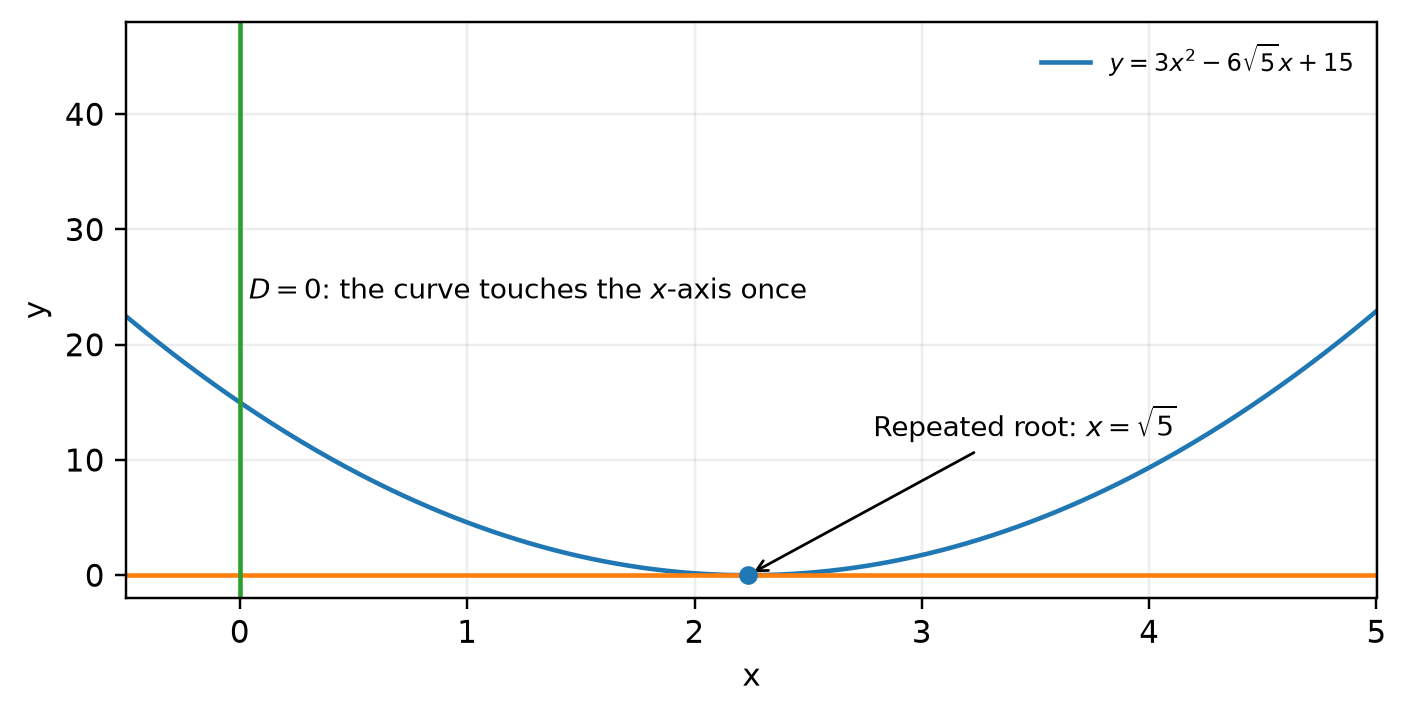
\includegraphics[width=0.92\linewidth]{../CBSE-2015-Class10-Updated-corrected_V3/figs/Q01_Quadratic.png}
\caption{At \(p=3\), the quadratic has a double root at \(x=\sqrt5\).}
\label{fig:q1-quadratic}
\end{figure}
\par\smallskip
\noindent\textbf{Code reference -}
\par\noindent\fbox{\parbox{\dimexpr\linewidth-2\fboxsep-2\fboxrule\relax}{\centering
\texttt{../CBSE-2015-Class10-Updated-corrected_V3/codes/Q01.py}}}

\setcounter{enumi}{1}\item A tower $AB$ is $20\,\mathrm m$ high and its shadow $BC$ is $20\sqrt3\,\mathrm m$ long. Find the Sun's altitude.
\begin{figure}[H]\centering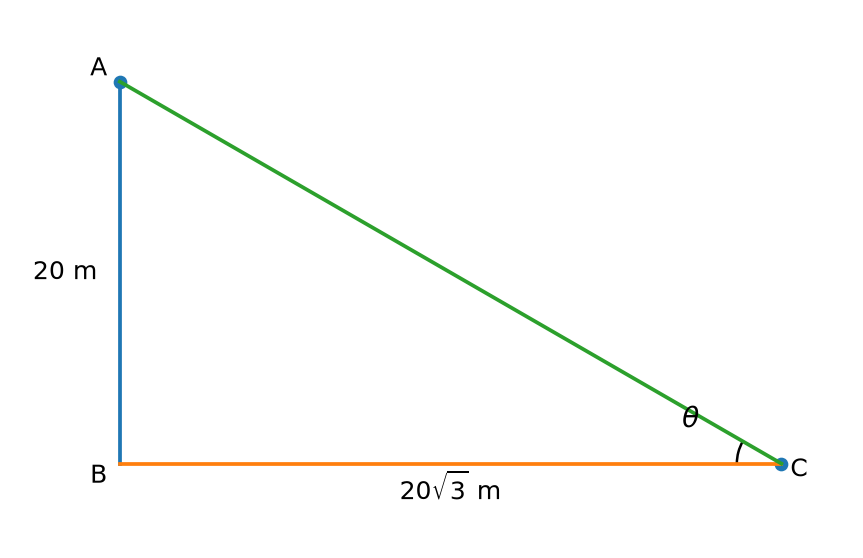
\includegraphics[width=0.78\linewidth]{../CBSE-2015-Class10-Updated-corrected_V3/figs/Tower.png}\caption{Tower and its shadow.}\label{fig:tower}\end{figure}
\solution Let the angle of elevation be $\theta$. From the right triangle,
\begin{equation*}
\tan\theta=\frac{AB}{BC}=\frac{20}{20\sqrt3}=\frac1{\sqrt3}\qquad\eqref{eq:trig-ratios}.
\end{equation*}
Thus $\theta=30^\circ$.



The tower-and-shadow diagram is generated by this script:
\par\smallskip
\noindent\textbf{Code reference -}
\par\noindent\fbox{\parbox{\dimexpr\linewidth-2\fboxsep-2\fboxrule\relax}{\centering\texttt{../CBSE-2015-Class10-Updated-corrected_V3/codes/Q02.py}}}
\par\smallskip
\newpage
\setcounter{enumi}{2}\item Two different dice are tossed together. Find the probability that the product of their top numbers is $6$.
\solution Let \(X,Y\) be the top numbers on the distinguishable dice.
They are independent discrete uniform random variables on
\(\{1,\ldots,6\}\), so \(P(X=i,Y=j)=1/36\). Define \(Z=XY\).
Its probability mass function is the push-forward of the joint law
under the map \((i,j)\mapsto ij\):
\[
p_Z(m)=P(Z=m)=
\sum_{i=1}^{6}\sum_{j=1}^{6}\frac1{36}\mathbf1_{\{ij=m\}}.
\]
The four ordered factor pairs producing \(m=6\) are
\((1,6),(2,3),(3,2),(6,1)\), so
\[
P(Z=6)=p_Z(6)=\frac4{36}=\boxed{\frac19}.
\]
The probability-generating function is
\[
G_Z(s)=E[s^Z]=\frac1{36}\sum_{i=1}^{6}\sum_{j=1}^{6}s^{ij};
\]
the coefficient of \(s^6\) is \(1/9\). Probability is conserved:
\[
\sum_m p_Z(m)=\frac1{36}
\sum_{i=1}^{6}\sum_{j=1}^{6}1=1.
\]
\begin{figure}[H]\centering
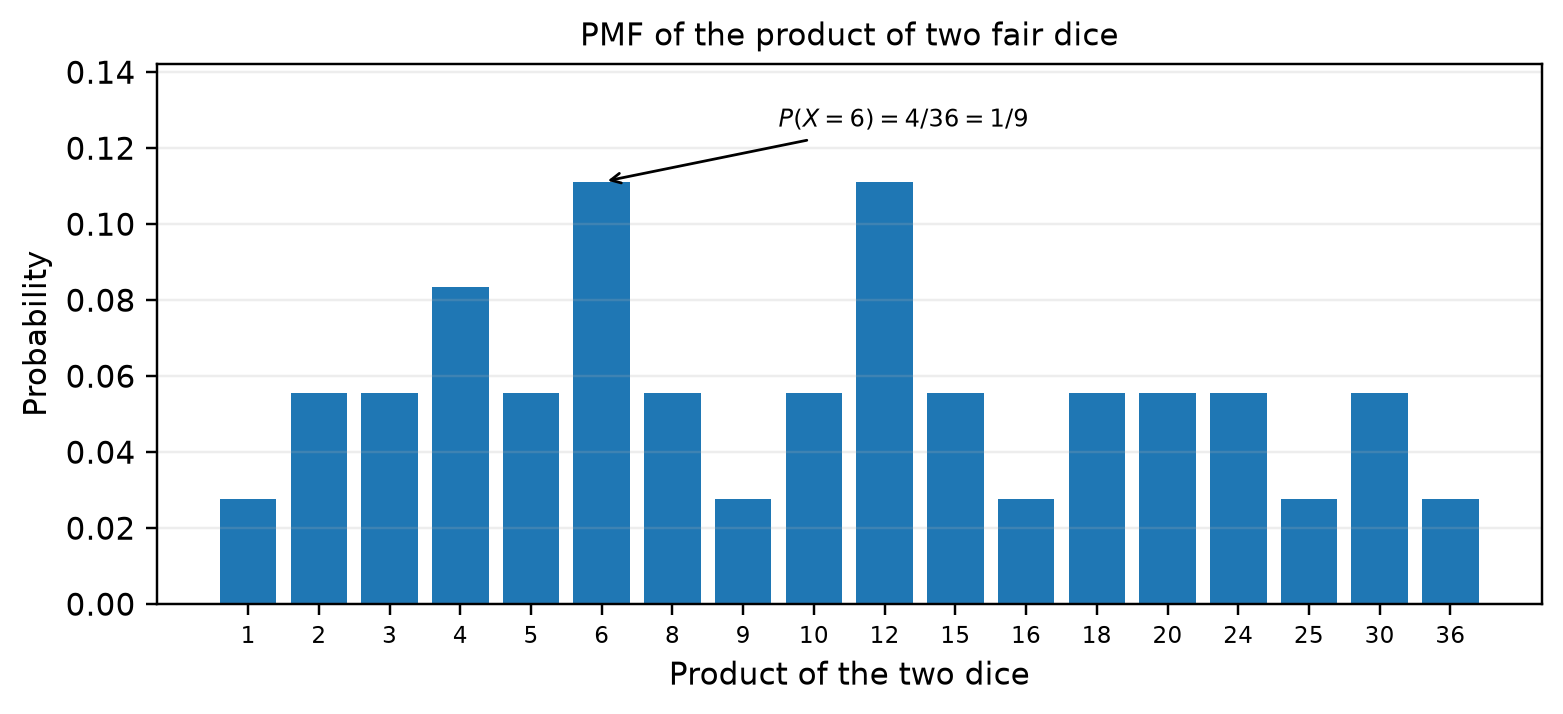
\includegraphics[width=0.98\linewidth]{../CBSE-2015-Class10-Updated-corrected_V3/figs/Q03_ProductPMF.png}
\caption{Push-forward probability mass function of the product of two fair dice.}
\label{fig:q3-pmf}
\end{figure}
\par\smallskip
\noindent\textbf{Code reference -}
\par\noindent\fbox{\parbox{\dimexpr\linewidth-2\fboxsep-2\fboxrule\relax}{\centering
\texttt{../CBSE-2015-Class10-Updated-corrected_V3/codes/Q03.py}}}

\newpage
\setcounter{enumi}{3}\item $PQ$ is a chord of a circle with centre $O$, and $PT$ is a tangent. If $\angle QPT=60^\circ$, find $\angle PRQ$.
\begin{figure}[H]\centering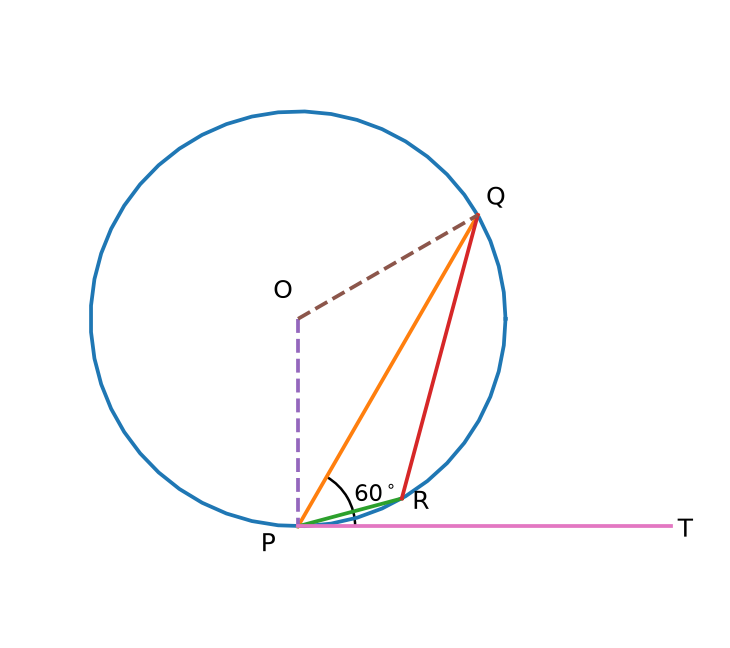
\includegraphics[width=0.72\linewidth]{../CBSE-2015-Class10-Updated-corrected_V3/figs/TangentChord.png}\caption{Chord--tangent configuration.}\label{fig:tangent-chord}\end{figure}
\solution Since $OP\perp PT$, we have $\angle OPQ=30^\circ$. As $OP=OQ$, triangle $OPQ$ is isosceles, so $\angle OQP=30^\circ$ and $\angle POQ=120^\circ$. With $R$ on the minor arc $PQ$, the intercepted major arc measures $240^\circ$. An angle at the circumference is half its intercepted arc, hence $\angle PRQ=120^\circ$. The tangent--chord theorem gives the alternate-segment angle as $60^\circ$, consistent with the supplementary angle here \qquad\eqref{eq:tangent-chord}.


The circle-and-tangent diagram is generated by this script:
\par\smallskip
\noindent\textbf{Code reference -}
\par\noindent\fbox{\parbox{\dimexpr\linewidth-2\fboxsep-2\fboxrule\relax}{\centering\texttt{../CBSE-2015-Class10-Updated-corrected_V3/codes/Q04.py}}}
\par\smallskip
\newpage
\setcounter{enumi}{5}\item A triangle circumscribes a circle of radius $3\,\mathrm{cm}$. The base portions are $BD=6\,\mathrm{cm}$ and $DC=9\,\mathrm{cm}$. If the triangle's area is $54\,\mathrm{cm}^2$, find $AB$ and $AC$.
\begin{figure}[H]\centering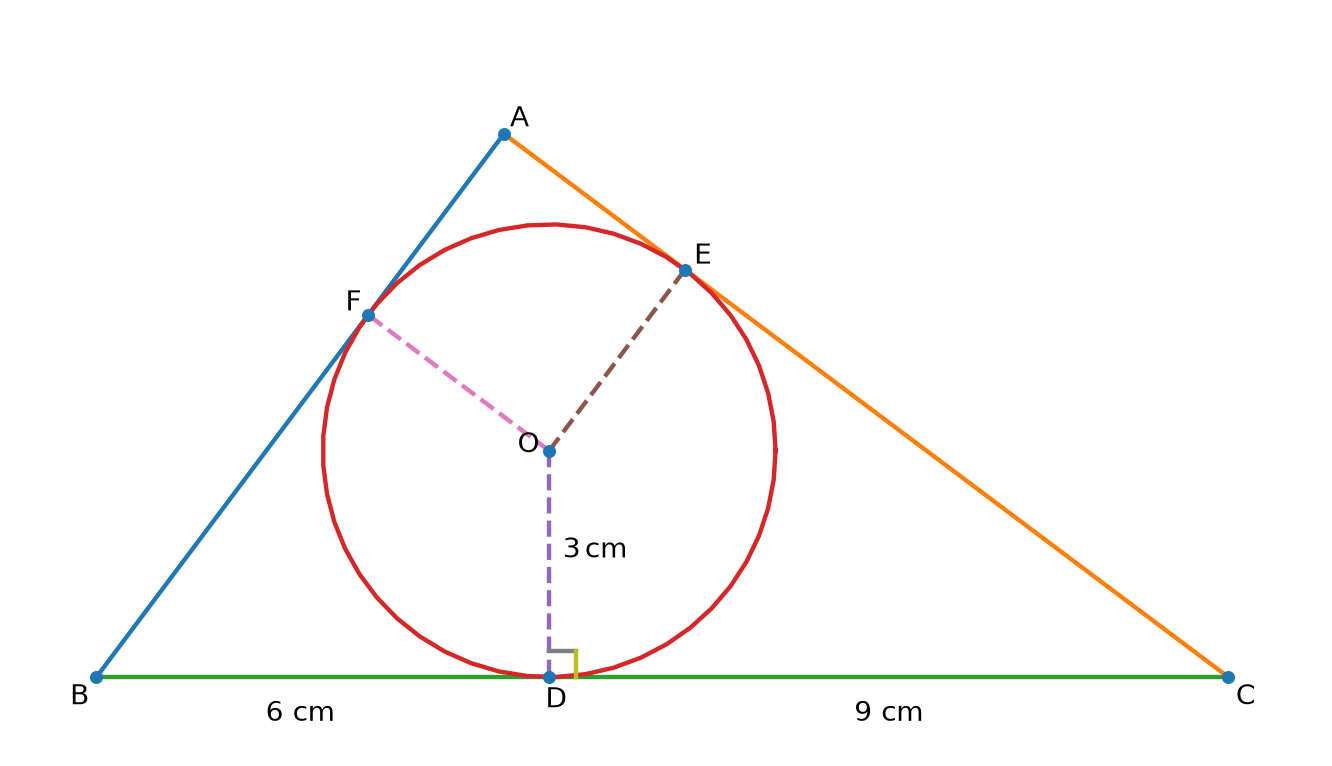
\includegraphics[width=0.78\linewidth]{../CBSE-2015-Class10-Updated-corrected_V3/figs/IncircleTriangle.png}\caption{Triangle with an incircle.}\label{fig:incircle}\end{figure}
\solution The semiperimeter is
\begin{equation*}
s=\frac{[ABC]}r=\frac{54}{3}=18\,\mathrm{cm}\qquad\eqref{eq:triangle-inradius}.
\end{equation*}
Tangents from a common external point have equal lengths. Let the tangent length from $A$ be $x$. Then $AB=x+6$, $AC=x+9$, and $BC=15$ \qquad\eqref{eq:equal-tangents}. Consequently,
\begin{equation*}
s=\frac{(x+6)+(x+9)+15}{2}=x+15=18,
\end{equation*}
so $x=3$. Therefore $AB=9\,\mathrm{cm},\quad AC=12\,\mathrm{cm}$.



The incircle diagram is generated by this script:
\par\smallskip
\noindent\textbf{Code reference -}
\par\noindent\fbox{\parbox{\dimexpr\linewidth-2\fboxsep-2\fboxrule\relax}{\centering\texttt{../CBSE-2015-Class10-Updated-corrected_V3/codes/Q06.py}}}
\par\smallskip
\newpage
\setcounter{enumi}{7}\item In an arithmetic progression, $S_5+S_7=167$ and $S_{10}=235$. Find the AP.
\solution Let \(x=(a,d)^T\). The conditions on the progression give
\[
Ax=b,\qquad A=\begin{pmatrix}12&31\\10&45\end{pmatrix},
\quad b=\begin{pmatrix}167\\235\end{pmatrix}.
\]
For \(A=D+L+U\), with \(D=\operatorname{diag}(12,45)\), the
Jacobi iteration is
\[
x^{(k+1)}=D^{-1}\bigl(b-(L+U)x^{(k)}\bigr)
=B_Jx^{(k)}+D^{-1}b,
\quad B_J=\begin{pmatrix}0&-31/12\\-2/9&0\end{pmatrix}.
\]
The characteristic equation is
\[
\lambda^2-\frac{31}{54}=0,\quad
\lambda_\pm=\pm\sqrt{\frac{31}{54}},\quad
\rho(B_J)=\sqrt{\frac{31}{54}}\approx0.757677<1.
\]
Thus Jacobi converges for every initial guess. Starting at
\(x^{(0)}=(0,0)^T\), the iterates converge to \(x^*=(1,5)^T\).
The residual norm \(\|Ax^{(k)}-b\|_2\) is approximately
\(1.121\), \(4.36\times10^{-3}\), \(1.69\times10^{-5}\), and
\(6.6\times10^{-8}\) after 20, 40, 60, and 80 iterations,
respectively. A suitable stopping rule requires both a small relative
iterate change and residual at most \(10^{-6}\). Therefore
\[
\boxed{a=1,\ d=5},\qquad 1,6,11,16,\ldots
\]
The negative eigenvalue explains the alternating component of
convergence; the verification script implements Jacobi directly.
\par\smallskip
\noindent\textbf{Code reference -}
\par\noindent\fbox{\parbox{\dimexpr\linewidth-2\fboxsep-2\fboxrule\relax}{\centering
\texttt{../CBSE-2015-Class10-Updated-corrected_V3/codes/Q08.py}}}

\setcounter{enumi}{8}\item $A(4,7)$, $B(p,3)$ and $C(7,3)$ form a right triangle, right-angled at $B$. Find $p$.
\solution The two side vectors meeting at $B$ are
\begin{equation*}
\overrightarrow{BA}=\myvec{4-p\\4},\qquad \overrightarrow{BC}=\myvec{7-p\\0}.
\end{equation*}
Since the sides are perpendicular, their inner product is zero:
\begin{equation*}
\langle\overrightarrow{BA},\overrightarrow{BC}\rangle=(4-p)(7-p)=0\qquad\eqref{eq:right-angle-dot}.
\end{equation*}
Thus $p=4$ or $p=7$. The second value makes $B=C$, so it does not form a triangle. Hence $p=4$.




\setcounter{enumi}{9}\item If $A(x,y)$, $B(-5,7)$ and $C(-4,5)$ are collinear, find the relation between $x$ and $y$.
\solution Place the three points in the homogeneous-coordinate matrix
\[
M=\begin{pmatrix}x&y&1\\-5&7&1\\-4&5&1\end{pmatrix}.
\]
Collinearity is equivalent to linear dependence of the three rows,
or \(\operatorname{rank}(M)\le2\). Since the last two points are
distinct, the rank is at least two; hence the condition is
\(\det M=0\). Subtracting the second row from the first and third gives
\[
\det M=
\begin{vmatrix}x+5&y-7\\1&-2\end{vmatrix}
=-2(x+5)-(y-7).
\]
Thus the required relation is
\[
\boxed{2x+y+3=0}.
]

\newpage
\setcounter{enumi}{10}\item The 14th term of an AP is twice its 8th term. If the 6th term is $-8$, find the sum of its first 20 terms.
\solution Represent the AP as the one-sided sequence
\(x[n]=a+(n-1)d\), \(n\ge1\), with \(x[0]=0\). Its unilateral
\(Z\)-transform is
\[
X(z)=\sum_{n=1}^{\infty}(a+(n-1)d)z^{-n}
=\frac{a}{z-1}+\frac{d}{(z-1)^2},\qquad |z|>1.
\]
The term constraints give \(a+13d=2(a+7d)\), so \(a+d=0\);
also \(a+5d=-8\). Thus \(a=2\) and \(d=-2\).
For the cumulative sequence \(s[n]=\sum_{k=1}^{n}x[k]\),
\[
S(z)=\frac{X(z)}{1-z^{-1}},
\]
the unilateral accumulation relation. Inverting it gives
\(s[n]=na+\frac{n(n-1)}2d\), so
\[
S_{20}=s[20]=20(2)+\frac{20\cdot19}{2}(-2)
=\boxed{-340}.
]

\setcounter{enumi}{12}\item An aeroplane is observed at an elevation of $60^\circ$ from point $A$. After 15 seconds, the elevation becomes $30^\circ$. If its altitude remains $1500\sqrt3\,\mathrm m$, find its speed in km/h.
\begin{figure}[H]\centering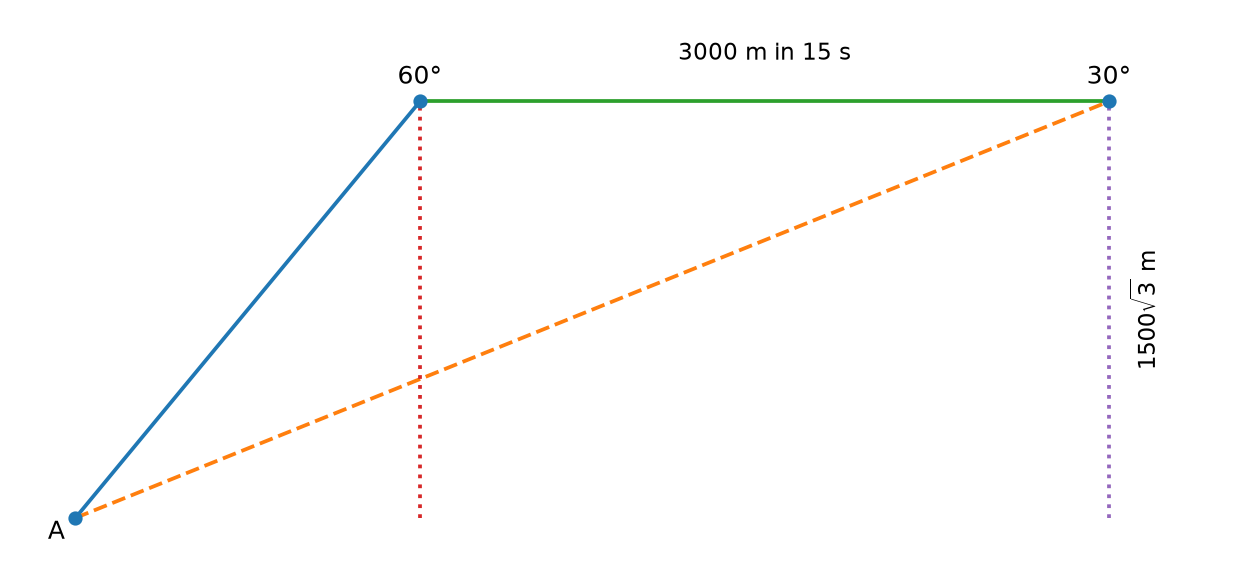
\includegraphics[width=0.86\linewidth]{../CBSE-2015-Class10-Updated-corrected_V3/figs/Aeroplane.png}\caption{The plane moves horizontally while staying at the same altitude.}\label{fig:aeroplane}\end{figure}
\solution Let its initial and final horizontal ranges be $x_1$ and $x_2$. Since the altitude $h$ is fixed, $x=h\cot\theta$:
\begin{align*}
x_1&=1500\sqrt3\cot60^\circ=1500\,\mathrm m,\\
x_2&=1500\sqrt3\cot30^\circ=4500\,\mathrm m\qquad\eqref{eq:horizontal-range}.
\end{align*}
The plane covers $x_2-x_1=3000\,\mathrm m$ in 15 s. Therefore,
\begin{equation*}
v=\frac{3000}{15}=200\,\mathrm{m/s}=200\times\frac{18}{5}=720\,\mathrm{km/h}\qquad\eqref{eq:speed-time}.
\end{equation*}



The speed calculation and accompanying figure are generated by this script:
\par\smallskip
\noindent\textbf{Code reference -}
\par\noindent\fbox{\parbox{\dimexpr\linewidth-2\fboxsep-2\fboxrule\relax}{\centering\texttt{../CBSE-2015-Class10-Updated-corrected_V3/codes/Q13.py}}}
\par\smallskip
\newpage
\setcounter{enumi}{13}\item $A(-2,-2)$ and $B(2,-4)$. Find the point $P$ on segment $AB$ for which $AP=\frac37 AB$.
\begin{figure}[H]\centering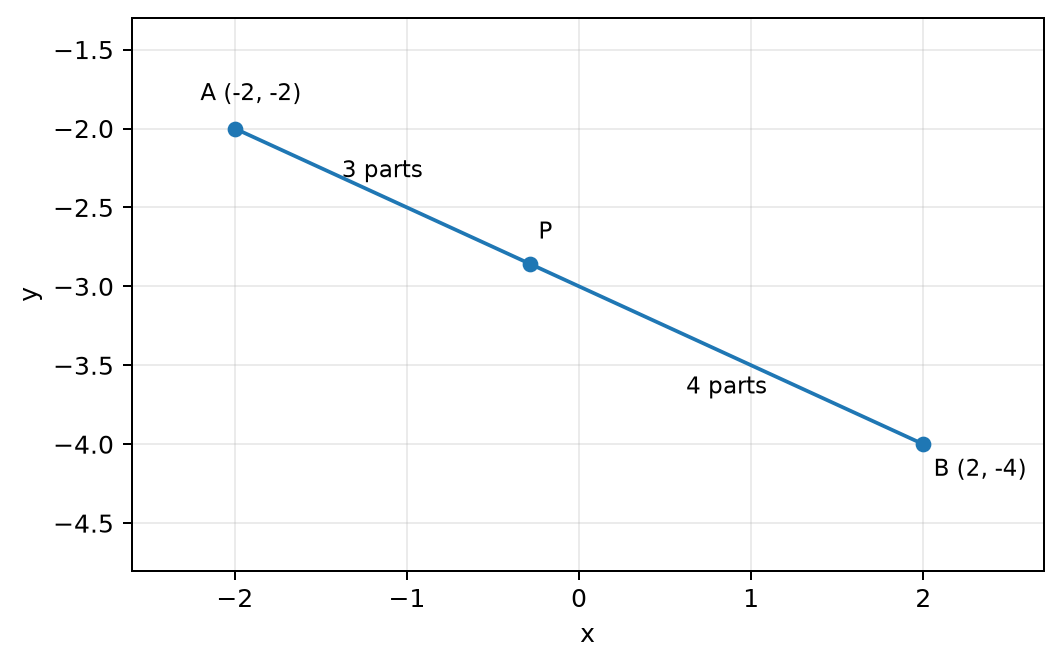
\includegraphics[width=0.82\linewidth]{../CBSE-2015-Class10-Updated-corrected_V3/figs/SectionPoint.png}\caption{The point $P$ is three-sevenths of the way from $A$ to $B$.}\label{fig:section-point}\end{figure}
\solution The section formula gives
\begin{align*}
\vec p&=\vec a+\frac37(\vec b-\vec a)\qquad\eqref{eq:vector-basics},\ \eqref{eq:section-vector}\\
&=\myvec{-2\\-2}+\frac37\myvec{4\\-2}=\myvec{-2/7\\-20/7}.
\end{align*}
Hence $P\left(-\frac27,-\frac{20}{7}\right)$.



The section-formula diagram is generated by this script:
\par\smallskip
\noindent\textbf{Code reference -}
\par\noindent\fbox{\parbox{\dimexpr\linewidth-2\fboxsep-2\fboxrule\relax}{\centering\texttt{../CBSE-2015-Class10-Updated-corrected_V3/codes/Q14.py}}}
\par\smallskip
\setcounter{enumi}{14}\item A jar contains only red, blue and orange balls. The probabilities of drawing a red and a blue ball are $\frac14$ and $\frac13$, respectively. If there are 10 orange balls, find the total number of balls.
\solution Let $N$ be the total number of balls. Write each probability separately:
\begin{align*}
P(R)&=\frac{\text{number of red balls}}{N}=\frac14,\\
P(B)&=\frac{\text{number of blue balls}}{N}=\frac13,\\
P(O)&=\frac{\text{number of orange balls}}{N}=\frac{10}{N}.
\end{align*}
Since every ball is one of these three colours, $P(R)+P(B)+P(O)=1\qquad\eqref{eq:three-events}$. Thus
\begin{equation*}
\frac14+\frac13+\frac{10}{N}=1\quad\Longrightarrow\quad\frac{10}{N}=\frac5{12}\quad\Longrightarrow\quad N=24.
\end{equation*}
So there are $24$ balls in total: 6 red, 8 blue and 10 orange.



\begin{figure}[H]\centering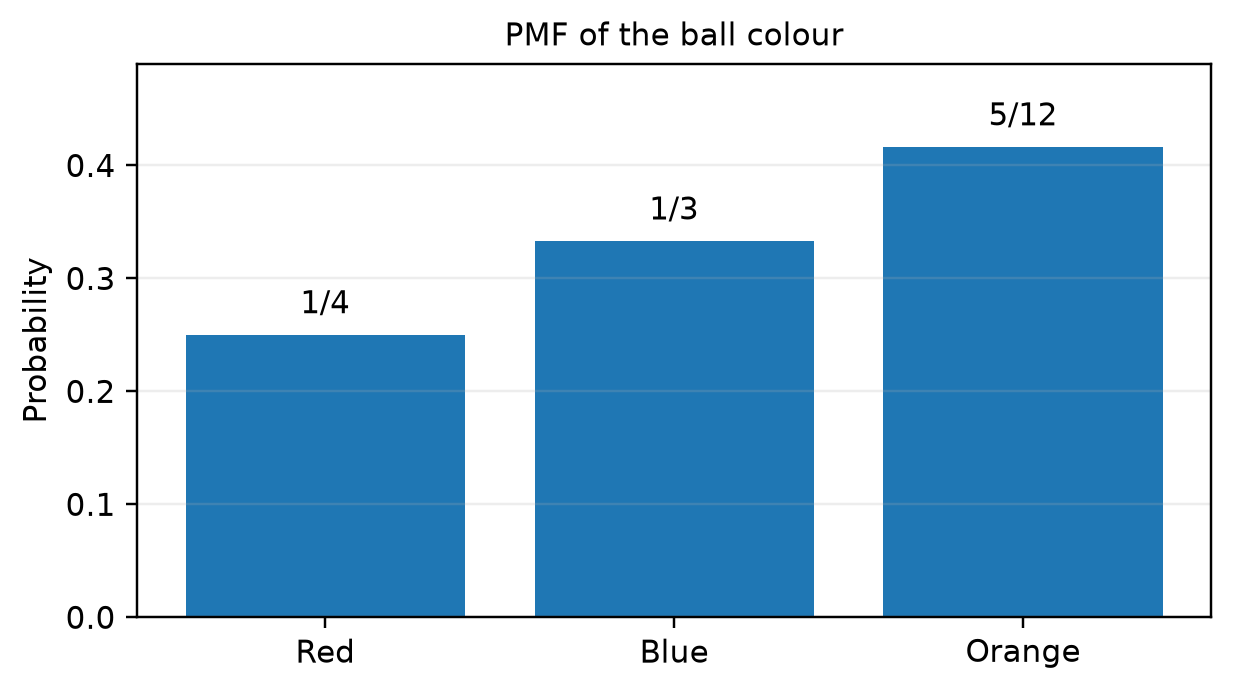
\includegraphics[width=0.9\linewidth]{../CBSE-2015-Class10-Updated-corrected_V3/figs/Q15_ColourPMF.png}\caption{Probability mass function for drawing each ball colour. The three probabilities sum to 1.}\label{fig:q15-pmf}\end{figure}
The Python code plots the theoretically derived probabilities $1/4$, $1/3$, and $5/12$ as a probability mass function:
\par\smallskip
\noindent\textbf{Code reference -}
\par\noindent\fbox{\parbox{\dimexpr\linewidth-2\fboxsep-2\fboxrule\relax}{\centering\texttt{../CBSE-2015-Class10-Updated-corrected_V3/codes/Q15.py}}}
\par\smallskip
\newpage
\setcounter{enumi}{15}\item Find the minor and major segment areas of a circle of radius $14\,\mathrm{cm}$ cut by a chord subtending $60^\circ$ at the centre. Use $\pi=\frac{22}{7}$.
\begin{figure}[H]\centering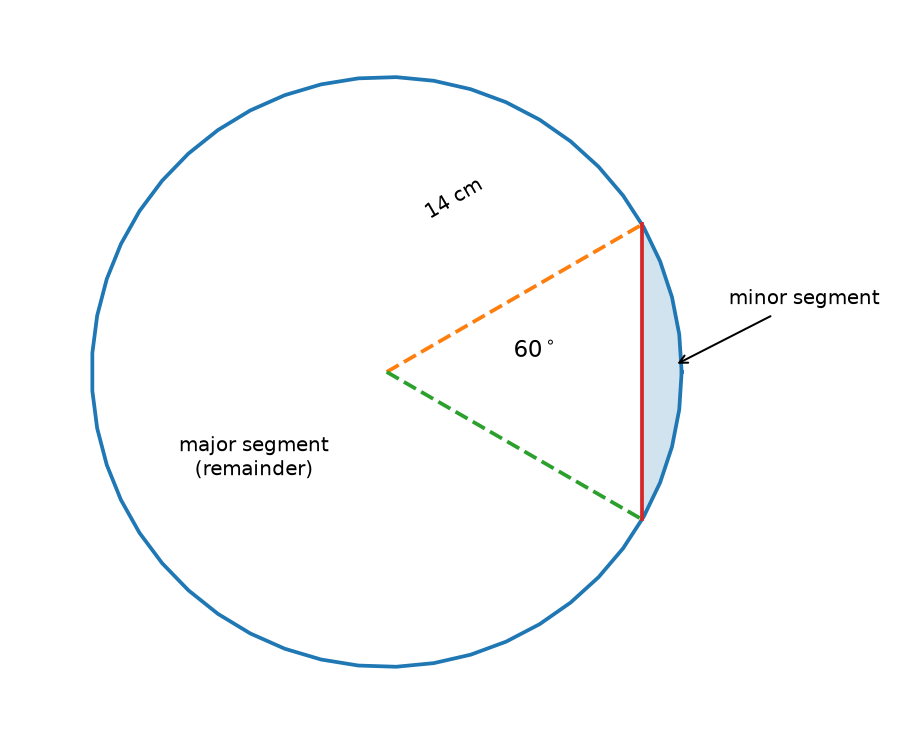
\includegraphics[width=0.86\linewidth]{../CBSE-2015-Class10-Updated-corrected_V3/figs/SegmentAreas.png}\caption{The minor segment is the small cap; the major segment is the remainder of the circle.}\label{fig:segment-areas}\end{figure}
\solution The sector angle is $60^\circ$, so
\begin{equation*}
A_{\mathrm{sector}}=\frac{60}{360}\pi(14)^2=\frac{308}{3}\,\mathrm{cm}^2\qquad\eqref{eq:sector-segment}.
\end{equation*}
The triangle between the two radii has two sides 14 cm and included angle $60^\circ$, so it is equilateral. Its area is $\frac{\sqrt3}{4}(14)^2=49\sqrt3\,\mathrm{cm}^2$. Subtracting this triangle from the sector gives
\begin{equation*}
A_{\mathrm{minor}}=\frac{308}{3}-49\sqrt3\,\mathrm{cm}^2.
\end{equation*}
The whole circle has area $\pi(14)^2=616\,\mathrm{cm}^2$. Therefore
\begin{equation*}
A_{\mathrm{major}}=616-A_{\mathrm{minor}}=\frac{1540}{3}+49\sqrt3\,\mathrm{cm}^2.
\end{equation*}



The segment diagram and area check are generated by this script:
\par\smallskip
\noindent\textbf{Code reference -}
\par\noindent\fbox{\parbox{\dimexpr\linewidth-2\fboxsep-2\fboxrule\relax}{\centering\texttt{../CBSE-2015-Class10-Updated-corrected_V3/codes/Q16.py}}}
\par\smallskip
\newpage
\setcounter{enumi}{16}\item One tent has a cylindrical lower part of diameter $4.2\,\mathrm m$ and height $4\,\mathrm m$, topped by a cone with the same diameter and height $2.8\,\mathrm m$. Canvas costs Rs. 100 per $\mathrm m^2$. Find the associations' 50\% contribution for 100 tents, and state the values shown.
\begin{figure}[H]\centering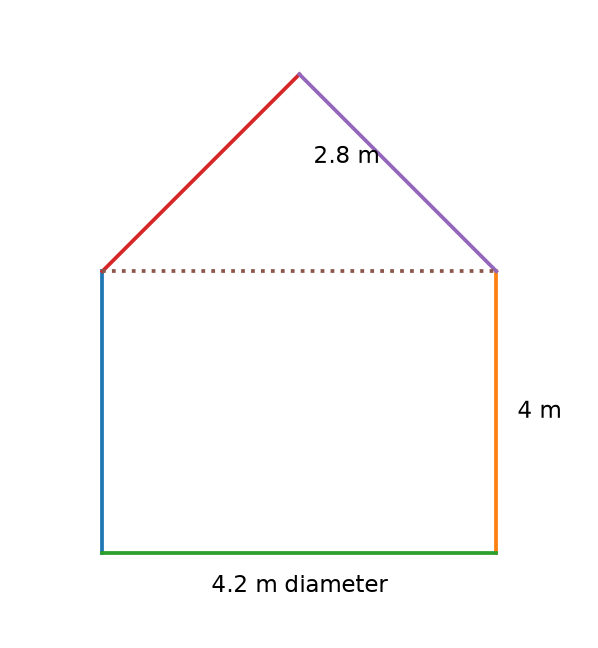
\includegraphics[width=0.72\linewidth]{../CBSE-2015-Class10-Updated-corrected_V3/figs/Tent.png}\caption{The tent consists of a cylinder and a cone and has no canvas floor.}\label{fig:tent}\end{figure}
\solution The radius is $r=2.1\,\mathrm m$. The cone's slant height is
\begin{equation*}
\ell=\sqrt{2.1^2+2.8^2}=3.5\,\mathrm m\qquad\eqref{eq:cone-formula}.
\end{equation*}
Only the curved cylinder and cone surfaces need canvas. Their combined area is
\begin{align*}
A&=2\pi rh+\pi r\ell\qquad\eqref{eq:cone-formula}\\
&=2\pi(2.1)(4)+\pi(2.1)(3.5)=75.9\,\mathrm m^2.
\end{align*}
For 100 tents, the total cost is $100\times75.9\times100=\text{Rs. }759{,}000$. Half is $\text{Rs. }379{,}500$. The plan also shows cooperation, initiative and care for people affected by floods.


The tent cross-section is generated by this script:
\par\smallskip
\noindent\textbf{Code reference -}
\par\noindent\fbox{\parbox{\dimexpr\linewidth-2\fboxsep-2\fboxrule\relax}{\centering\texttt{../CBSE-2015-Class10-Updated-corrected_V3/codes/Q17.py}}}
\par\smallskip
\setcounter{enumi}{21}\item Find the 60th term of the AP $8,10,12,\ldots$ and the sum of its last 10 terms.
\solution Here $a=8$ and $d=2$.
\begin{equation*}
t_{60}=8+59(2)=126\qquad\eqref{eq:ap}.
\end{equation*}
The 51st term is $t_{51}=8+50(2)=108$. The last ten terms run from 108 to 126, so
\begin{equation*}
S_{51\ldots60}=S_{60}-S_{50}=\frac{10}{2}(108+126)=1170\qquad\eqref{eq:ap-subsum}.
\end{equation*}



The 60th term and final-ten-term sum are checked by this script:
\par\smallskip
\noindent\textbf{Code reference -}
\par\noindent\fbox{\parbox{\dimexpr\linewidth-2\fboxsep-2\fboxrule\relax}{\centering\texttt{../CBSE-2015-Class10-Updated-corrected_V3/codes/Q22.py}}}
\par\smallskip
\setcounter{enumi}{26}\item Point $A$ is 20 m above a lake. The angle of elevation of a cloud is $30^\circ$, while the angle of depression of its reflection in the lake is $60^\circ$. Find the distance from $A$ to the cloud.
\begin{figure}[H]\centering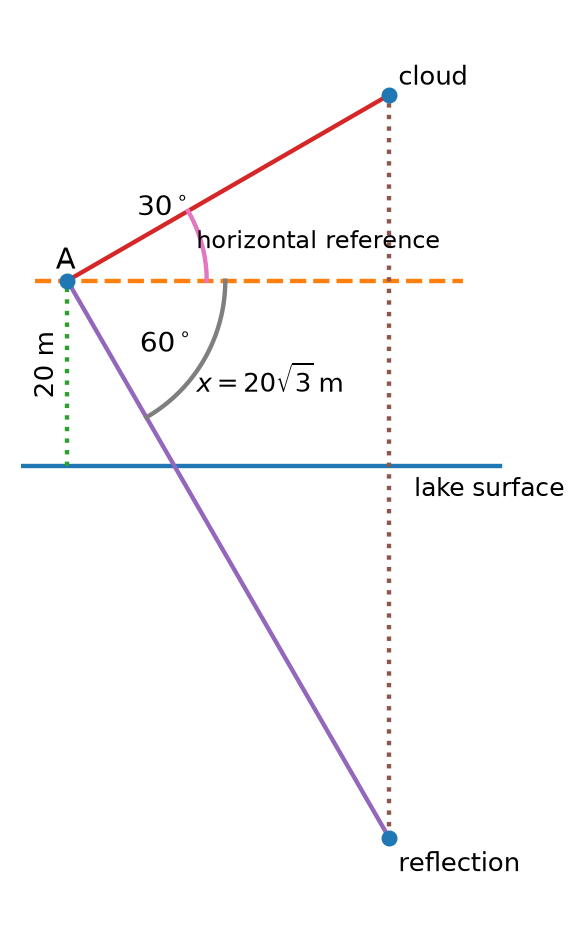
\includegraphics[height=0.42\textheight,keepaspectratio]{../CBSE-2015-Class10-Updated-corrected_V3/figs/CloudReflection.png}\caption{The reflection is as far below the lake surface as the cloud is above it.}\label{fig:cloud-reflection}\end{figure}
\solution Let $H$ be the cloud's height above the lake and let $x$ be the horizontal distance from $A$ to the vertical line through the cloud. The cloud is $H-20$ metres above $A$, while its reflection is $H+20$ metres below $A$. As shown in the figure, both the angle of elevation and the angle of depression are measured from the horizontal reference line through $A$. Using the two angles,
\begin{align*}
\frac{H-20}{x}&=\tan30^\circ=\frac1{\sqrt3},\\
\frac{H+20}{x}&=\tan60^\circ=\sqrt3.\qquad\eqref{eq:trig-ratios},\ \eqref{eq:horizontal-range}
\end{align*}
Rearranging produces a linear system in the unknowns $H$ and $x$:
\begin{equation*}
\myvec{1&-1/\sqrt3\\1&-\sqrt3}\myvec{H\\x}=\myvec{20\\-20}.
\end{equation*}
For clarity, solve this system by Gaussian elimination. Its augmented matrix is
\begin{equation*}
\left[\begin{array}{cc|c}1&-1/\sqrt3&20\\1&-\sqrt3&-20\end{array}\right]
\xrightarrow{\;R_2\leftarrow R_2-R_1\;}
\left[\begin{array}{cc|c}1&-1/\sqrt3&20\\0&-2/\sqrt3&-40\end{array}\right].
\end{equation*}
The second row gives $-2x/\sqrt3=-40$, so $x=20\sqrt3\,\mathrm m$. Substitution into the first row yields $H-20=20$, so $H=40\,\mathrm m$. Hence the vertical separation between $A$ and the cloud is $H-20=20\,\mathrm m$. By Pythagoras,
\begin{equation*}
AC=\sqrt{x^2+(H-20)^2}=\sqrt{(20\sqrt3)^2+20^2}=40\,\mathrm m.
\end{equation*}



The linear system is solved independently and the angle diagram is generated by this script:
\par\smallskip
\noindent\textbf{Code reference -}
\par\noindent\fbox{\parbox{\dimexpr\linewidth-2\fboxsep-2\fboxrule\relax}{\centering\texttt{../CBSE-2015-Class10-Updated-corrected_V3/codes/Q27.py}}}
\par\smallskip
\setcounter{enumi}{27}\item A card is drawn from a well-shuffled 52-card deck. Find the probability that it is (i) a spade or an ace, (ii) a black king, (iii) neither a jack nor a king, (iv) either a king or a queen.
\solution Use the classical probability and union rules:
\begin{enumerate}[label=(\roman*)]
\item The 13 spades and 4 aces overlap at the ace of spades. Thus $P=(13+4-1)/52=4/13\qquad\eqref{eq:prob-classical}, \eqref{eq:prob-union}$.
\item There are two black kings, so $P=2/52=1/26\qquad\eqref{eq:prob-classical}$.
\item There are four jacks and four kings. Their complement contains $52-4-4=44$ cards, so $P=44/52=11/13\qquad\eqref{eq:prob-classical}$.
\item Kings and queens are disjoint categories, each with four cards. Thus $P=(4+4)/52=2/13\qquad\eqref{eq:prob-classical}$.
\end{enumerate}

\setcounter{enumi}{28}\item Find $k$ if the triangle with vertices $(1,-1)$, $(-4,2k)$ and $(-k,-5)$ has area 24 square units.
\solution Taking differences of the coordinate vectors,
\begin{equation*}
2[ABC]=\left|\mydet{-5&2k+1\\-k-1&-4}\right|\qquad\eqref{eq:triangle-det}.
\end{equation*}
Expanding the determinant gives
\begin{equation*}
2[ABC]=|2k^2+3k+21|.
\end{equation*}
Since $2k^2+3k+21$ has positive leading coefficient and discriminant $9-168=-159<0$, it is positive for every real $k$. The specified area is 24, so the determinant's absolute value is 48 and
\begin{equation*}
2k^2+3k+21=48\quad\Longrightarrow\quad2k^2+3k-27=0.
\end{equation*}
Applying the quadratic formula, the discriminant is $3^2-4(2)(-27)=225$, hence
\begin{equation*}
k=\frac{-3\pm\sqrt{225}}4=\frac{-3\pm15}4.
\end{equation*}
Therefore both solutions are valid: $k=3\quad\text{or}\quad k=-\frac92$.



\begin{figure}[H]\centering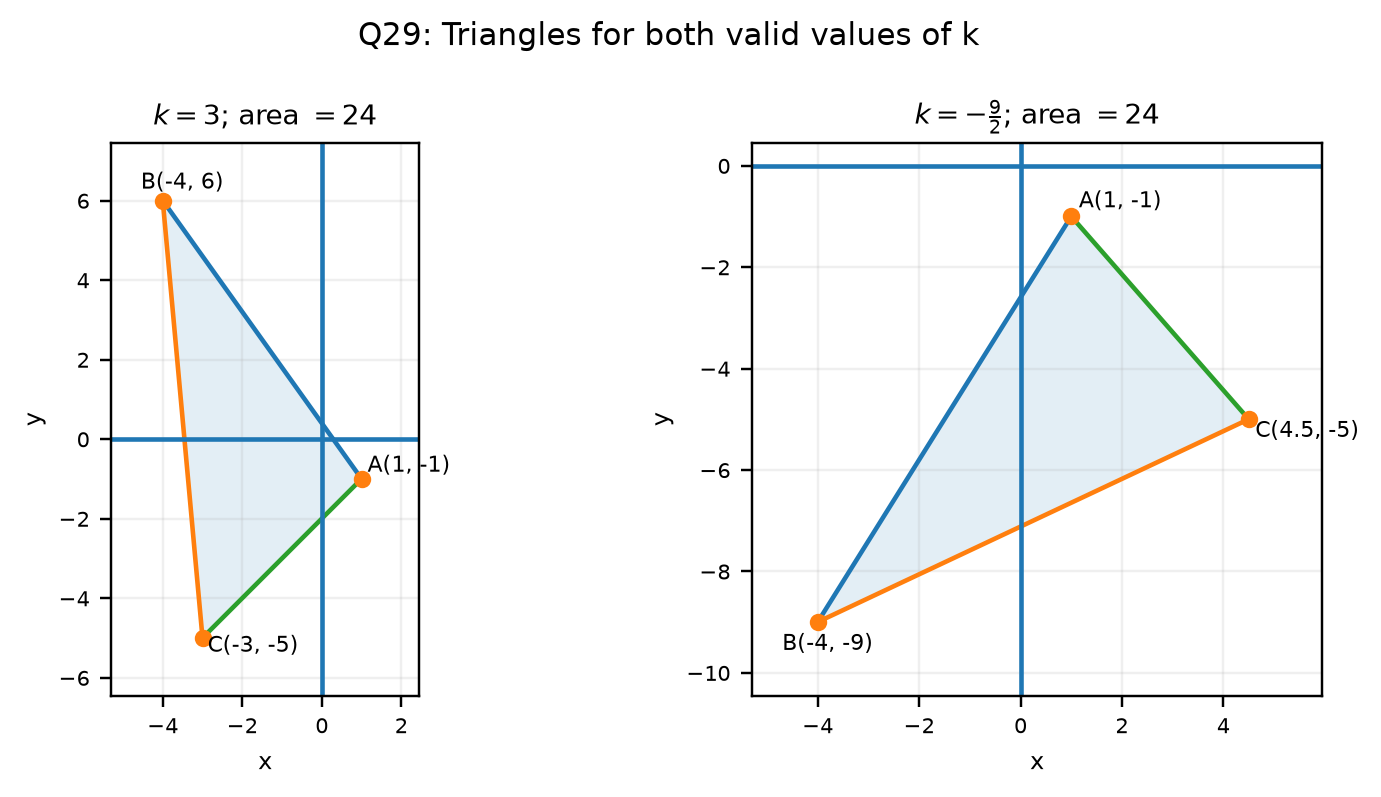
\includegraphics[width=0.99\linewidth]{../CBSE-2015-Class10-Updated-corrected_V3/figs/Q29_Triangles.png}\caption{The triangle formed by the given coordinates for each valid solution, $k=3$ and $k=-\frac92$. Both triangles have area 24 square units.}\label{fig:q29-triangles}\end{figure}
The Python code plots the triangles for the two theoretically derived values of $k$, using the coordinate area formula for the displayed areas:
\par\smallskip
\noindent\textbf{Code reference -}
\par\noindent\fbox{\parbox{\dimexpr\linewidth-2\fboxsep-2\fboxrule\relax}{\centering\texttt{../CBSE-2015-Class10-Updated-corrected_V3/codes/Q29.py}}}
\par\smallskip
\setcounter{enumi}{29}\item A square lawn has side 42 m. Two circular flower beds lie outside the vertical sides, with each circle centred at the intersection $O$ of the square's diagonals. Find the total shaded area. Use $\pi=22/7$.
\begin{figure}[H]\centering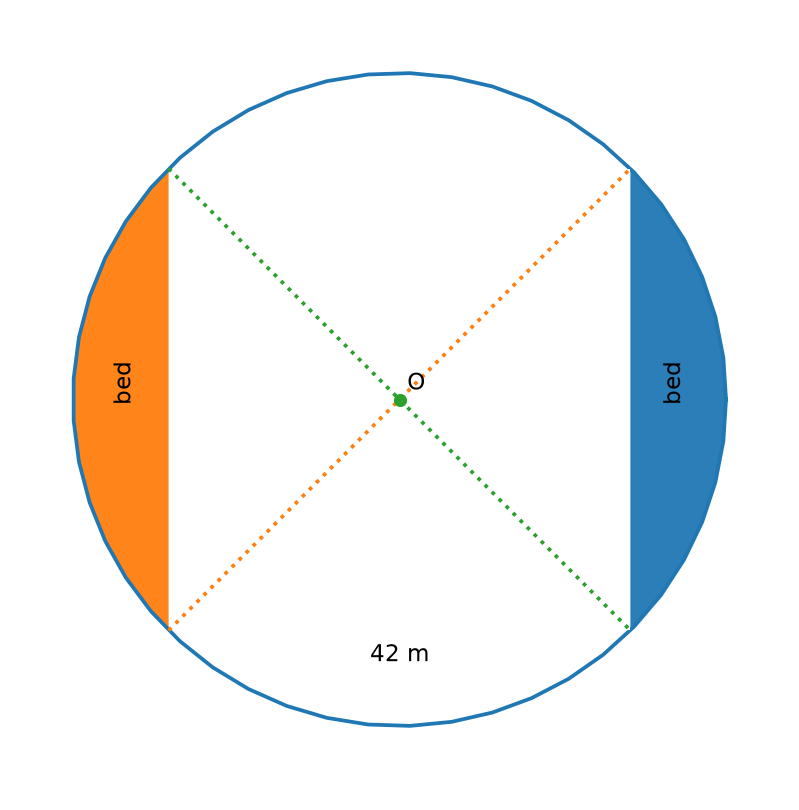
\includegraphics[width=0.84\linewidth]{../CBSE-2015-Class10-Updated-corrected_V3/figs/FlowerBeds.png}\caption{The shaded parts are the two circular segments outside the square lawn.}\label{fig:flower-beds}\end{figure}
\solution The radius from the centre to a corner is half the diagonal. Thus
\begin{equation*}
r^2=\frac{42^2+42^2}{4}=882\,\mathrm{m}^2.
\end{equation*}
Each vertical side subtends $90^\circ$ at $O$. The area of one segment is the area of a quarter-circle sector minus the right triangle with legs 21 m and 21 m:
\begin{equation*}
A_1=\frac14\pi r^2-\frac12(42/2)^2=\frac{882\pi}{4}-441.
\end{equation*}
The two beds are congruent, so
\begin{equation*}
A_{\mathrm{total}}=2A_1=441\pi-882\qquad\eqref{eq:shaded-area}.
\end{equation*}
Using $\pi=22/7$ gives $A_{\mathrm{total}}=1386-882=504\,\mathrm{m}^2$.



The flower-bed figure and shaded-area result are generated by this script:
\par\smallskip
\noindent\textbf{Code reference -}
\par\noindent\fbox{\parbox{\dimexpr\linewidth-2\fboxsep-2\fboxrule\relax}{\centering\texttt{../CBSE-2015-Class10-Updated-corrected_V3/codes/Q30.py}}}
\par\smallskip
\setcounter{enumi}{30}\item From both ends of a metal cylinder, hemispherical cavities of the same diameter are scooped out. The cylinder has height 10 cm and radius 4.2 cm. The remaining metal is made into a cylindrical wire of thickness 1.4 cm. Find the wire length. Use $\pi=22/7$.
\begin{figure}[H]\centering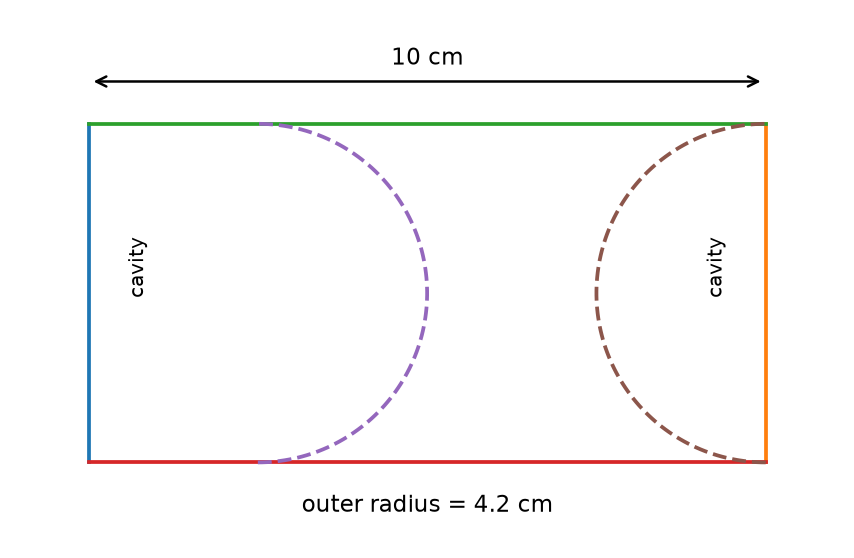
\includegraphics[width=0.84\linewidth]{../CBSE-2015-Class10-Updated-corrected_V3/figs/CylinderScooped.png}\caption{Two hemispherical cavities remove the volume of one sphere.}\label{fig:cylinder-scooped}\end{figure}
\solution The two hemispherical cavities together have the volume of one sphere. The remaining metal has volume
\begin{equation*}
V=\pi(4.2)^2(10)-\frac43\pi(4.2)^3=77.616\pi\,\mathrm{cm}^3\qquad\eqref{eq:cylinder-formula},\ \eqref{eq:sphere-formula},\ \eqref{eq:scooped-cylinder}.
\end{equation*}
The wire's thickness is its diameter, so its radius is $0.7$ cm. Equating the volumes gives
\begin{equation*}
\pi(0.7)^2L=77.616\pi\quad\Longrightarrow\quad L=\frac{77.616}{0.49}=158.4\,\mathrm{cm}.
\end{equation*}


The cylinder-and-cavities diagram is generated by this script:
\par\smallskip
\noindent\textbf{Code reference -}
\par\noindent\fbox{\parbox{\dimexpr\linewidth-2\fboxsep-2\fboxrule\relax}{\centering\texttt{../CBSE-2015-Class10-Updated-corrected_V3/codes/Q31.py}}}
\par\smallskip\end{enumerate}


\newpage
\section{CBSE Class 12 Mathematics 2015}
\subsection{Formulae}
\paragraph*{Formulae referenced in the problems}\par
\begin{enumerate}[label=\theenumi,leftmargin=4mm,itemsep=4pt]
\setcounter{enumi}{0}\item

\begin{equation}
\vec a\times\vec b=
\begin{pmatrix}
a_2b_3-a_3b_2\\
a_3b_1-a_1b_3\\
a_1b_2-a_2b_1
\end{pmatrix}.
\label{eq:cross-product}
\end{equation}
\begin{equation}
\vec a\times\vec b\perp\vec a,\qquad
\vec a\times\vec b\perp\vec b.
\label{eq:cross-perpendicular}
\end{equation}

\setcounter{enumi}{4}\item

\begin{equation}
\vec a\cdot\vec b=a_1b_1+a_2b_2+a_3b_3,\qquad
\vec a\perp\vec b\iff\vec a\cdot\vec b=0.
\label{eq:dot-product}
\end{equation}

\setcounter{enumi}{5}\item

\begin{equation}
d(\text{parallel lines})=
\frac{\norm{(\vec b-\vec a)\times\vec v}}{\norm{\vec v}}.
\label{eq:parallel-distance}
\end{equation}

\setcounter{enumi}{9}\item

\begin{align}
\text{line parallel to plane}&\iff \vec d\cdot\vec n=0.
\label{eq:line-plane-parallel}\\
\text{plane through }\vec r_0\text{ with normal }\vec n:\quad
\vec n\cdot(\vec r-\vec r_0)&=0.
\label{eq:plane-normal}
\end{align}

\setcounter{enumi}{14}\item

\begin{equation}
\vec r=\vec A+t\vec d
\quad\text{for a line through }\vec A\text{ with direction }\vec d.
\label{eq:line-point-direction}
\end{equation}

\setcounter{enumi}{21}\item

\begin{equation}
y=vx\quad\Longrightarrow\quad y'=v+xv'
\quad\text{(homogeneous first-order ODE)}.
\label{eq:homogeneous-substitution}
\end{equation}

\setcounter{enumi}{23}\item

\begin{equation}
\mu(x)=e^{\int P(x)\,dx}.
\label{eq:if-24}
\end{equation}

\setcounter{enumi}{24}\item

\begin{equation}
\frac{d}{dx}\log|u(x)|=\frac{u'(x)}{u(x)},\qquad u(x)\ne0.
\label{eq:log-derivative-25}
\end{equation}

\setcounter{enumi}{27}\item

\begin{equation}
\det(AB)=\det(A)\det(B),\qquad
\det(A^n)=(\det A)^n.
\label{eq:det-power}
\end{equation}

\setcounter{enumi}{29}\item

\begin{equation}
A^{-1}=\frac{\operatorname{adj}(A)}{\det A},\qquad \det A\ne0.
\label{eq:inverse-matrix}
\end{equation}

\setcounter{enumi}{35}\item

\begin{equation}
a^2+b^2+c^2-ab-bc-ca
=\frac12\bigl((a-b)^2+(b-c)^2+(c-a)^2\bigr).
\label{eq:sum-squares}
\end{equation}

\setcounter{enumi}{36}\item

\begin{equation}
[A\mid\vec b]\xrightarrow{\text{elementary row operations}}[I\mid\vec x]
\quad\text{(Gaussian elimination)}.
\label{eq:gaussian-elimination}
\end{equation}

\setcounter{enumi}{37}\item

\begin{align}
\int\frac{du}{a^2+u^2}&=\frac1a\tan^{-1}\left(\frac{u}{a}\right)+C
\label{eq:scaled-arctan-integral-38}\\
\int\frac{du}{1+u^2}&=\tan^{-1}u+C.
\label{eq:arctan-integral-38}
\end{align}

\setcounter{enumi}{38}\item

\begin{equation}
\int\frac{du}{a^2-u^2}
=\frac1{2a}\log\left|\frac{a+u}{a-u}\right|+C.
\label{eq:int-rational-39}
\end{equation}

\setcounter{enumi}{39}\item

\begin{equation}
\frac{d}{dx}\log|u(x)|=\frac{u'(x)}{u(x)},\qquad u(x)\ne0.
\label{eq:log-derivative-40}
\end{equation}

\setcounter{enumi}{40}\item

\begin{equation}
\frac{P(x)}{(x-a)(x^2+b^2)}
=Q(x)+\frac{A}{x-a}+\frac{Bx+C}{x^2+b^2}.
\label{eq:partial-fractions-41}
\end{equation}

\setcounter{enumi}{41}\item

\begin{equation}
\frac{d}{dx}\log|u(x)|=\frac{u'(x)}{u(x)},\qquad u(x)\ne0.
\label{eq:log-derivative-42}
\end{equation}

\setcounter{enumi}{42}\item

\begin{equation}
\frac{P(x)}{(x-a)(x^2+b^2)}
=Q(x)+\frac{A}{x-a}+\frac{Bx+C}{x^2+b^2}.
\label{eq:partial-fractions-43}
\end{equation}

\setcounter{enumi}{43}\item

\begin{equation}
\frac{5\sin x+3\cos x}{\sin x+\cos x}
=4+\frac{\sin x-\cos x}{\sin x+\cos x}.
\label{eq:trig-split-44}
\end{equation}

\setcounter{enumi}{45}\item

\begin{equation}
A=\int_a^b|y_{\mathrm{upper}}-y_{\mathrm{lower}}|\,dx.
\label{eq:area-between-46}
\end{equation}

\setcounter{enumi}{46}\item

\begin{equation}
A=\int_a^b|y_{\mathrm{upper}}-y_{\mathrm{lower}}|\,dx.
\label{eq:area-between-47}
\end{equation}

\setcounter{enumi}{47}\item

\begin{equation}
\lim_{x\to a^-}f(x)=f(a)=\lim_{x\to a^+}f(x),\qquad
f'_{-}(a)=f'_{+}(a)=f'(a).
\label{eq:continuity-differentiability-48}
\end{equation}

\setcounter{enumi}{48}\item

\begin{equation}
\begin{aligned}
\text{reflexive: }&(a,a)\in R,\\
\text{symmetric: }&(a,b)\in R\Rightarrow(b,a)\in R,\\
\text{transitive: }&(a,b),(b,c)\in R\Rightarrow(a,c)\in R.
\end{aligned}
\label{eq:relation-properties-49}
\end{equation}

\setcounter{enumi}{49}\item

\begin{equation}
\text{For componentwise addition on }\mathbb R^2:\quad
e=(0,0),\quad(a,b)^{-1}=(-a,-b).
\label{eq:componentwise-operation-50}
\end{equation}

\setcounter{enumi}{50}\item

\begin{equation}
a*b=(a+b)\bmod n,\quad
0\text{ is the identity},\quad
(-a)\bmod n\text{ is the additive inverse}.
\label{eq:modular-operation-51}
\end{equation}

\setcounter{enumi}{51}\item

\begin{equation}
\lim_{x\to a^-}f(x)=f(a)=\lim_{x\to a^+}f(x).
\label{eq:continuity-limits-52}
\end{equation}

\setcounter{enumi}{52}\item

\begin{align}
X\sim\operatorname{Bin}(n,p):\quad
P(X=k)&=\binom nkp^k(1-p)^{n-k}.
\label{eq:binomial-53}\\
G(z)&=\sum_jP(D=j)z^j.
\label{eq:walk-pgf}
\end{align}

\setcounter{enumi}{53}\item

\begin{align}
P(A\mid E)&=\frac{P(E\mid A)P(A)}{P(E)}.
\label{eq:bayes-54}\\
P(E)&=\sum_iP(E\mid A_i)P(A_i).
\label{eq:total-probability-54}
\end{align}

\setcounter{enumi}{54}\item

\begin{align}
E[X]&=\sum_x xP(X=x),\quad
\operatorname{Var}(X)=E[X^2]-E[X]^2.
\label{eq:mean-variance-55}\\
P(X=k)&=\frac{\binom Kk\binom{N-K}{n-k}}{\binom Nn}.
\label{eq:hypergeometric-55}
\end{align}

\setcounter{enumi}{55}\item

\begin{equation}
P(X=k)=\binom nkp^k(1-p)^{n-k}.
\label{eq:binomial-56}
\end{equation}

\setcounter{enumi}{56}\item

\begin{equation}
P(E)=\sum_iP(E\mid A_i)P(A_i).
\label{eq:total-probability-57}
\end{equation}

\setcounter{enumi}{58}\item

\begin{equation}
\text{Evaluate the objective at each feasible corner; an optimum occurs at a feasible vertex.}
\label{eq:lpp-59}
\end{equation}

\setcounter{enumi}{59}\item

\begin{equation}
\text{LPP optimum}=\text{best objective value among feasible vertices}.
\label{eq:lpp-60}
\end{equation}

\setcounter{enumi}{63}\item

\begin{equation}
x\cos\theta+y\sin\theta=r.
\label{eq:circle-tangent-64}
\end{equation}

\setcounter{enumi}{64}\item

\begin{equation}
\text{ellipse point }(a\cos t,b\sin t),\qquad
A_{\triangle}=\frac12 bh.
\label{eq:ellipse-area-65}
\end{equation}
\end{enumerate}

\newpage
\subsection{Problems}
% This document follows the topic-organised question collection in
% gadepall/cbse-papers/2015/math/12/main.tex. Obvious transcription errors are
% corrected in the question text where the intended statement is unambiguous.
\paragraph*{Vectors and three-dimensional geometry}
\begin{enumerate}[label=\theenumi,leftmargin=4mm,itemsep=9pt]
\setcounter{enumi}{0}\item Find a vector of magnitude $\sqrt{171}$ perpendicular to both $\vec a=\myvec{1\\-2\\-3}$ and $\vec b=\myvec{3\\-1\\-2}$.
\solution Perpendicularity defines a homogeneous linear system in the unknown
vector \(v\):
\[
Av=0,\qquad
A=\begin{pmatrix}1&-2&-3\\3&-1&-2\end{pmatrix}.
\]
The two rows are independent, so \(\operatorname{rank}(A)=2\).
By the rank--nullity theorem,
\[
\dim\ker A=3-\operatorname{rank}(A)=1.
\]
Solving the two homogeneous equations gives a null-space basis
\[
n=\begin{pmatrix}1\\-7\\5\end{pmatrix},
\qquad \|n\|=\sqrt{75}=5\sqrt3.
\]
Every vector perpendicular to both given vectors is a scalar
multiple of \(n\). Scaling to the prescribed magnitude gives
\[
v=\pm\frac{\sqrt{171}}{5\sqrt3}n
=\boxed{\pm\frac{\sqrt{57}}5
\begin{pmatrix}1\\-7\\5\end{pmatrix}}.
\]
An SVD is useful only as a numerical rank/null-space check; the exact
null-space calculation determines the answer.
\begin{figure}[H]\centering
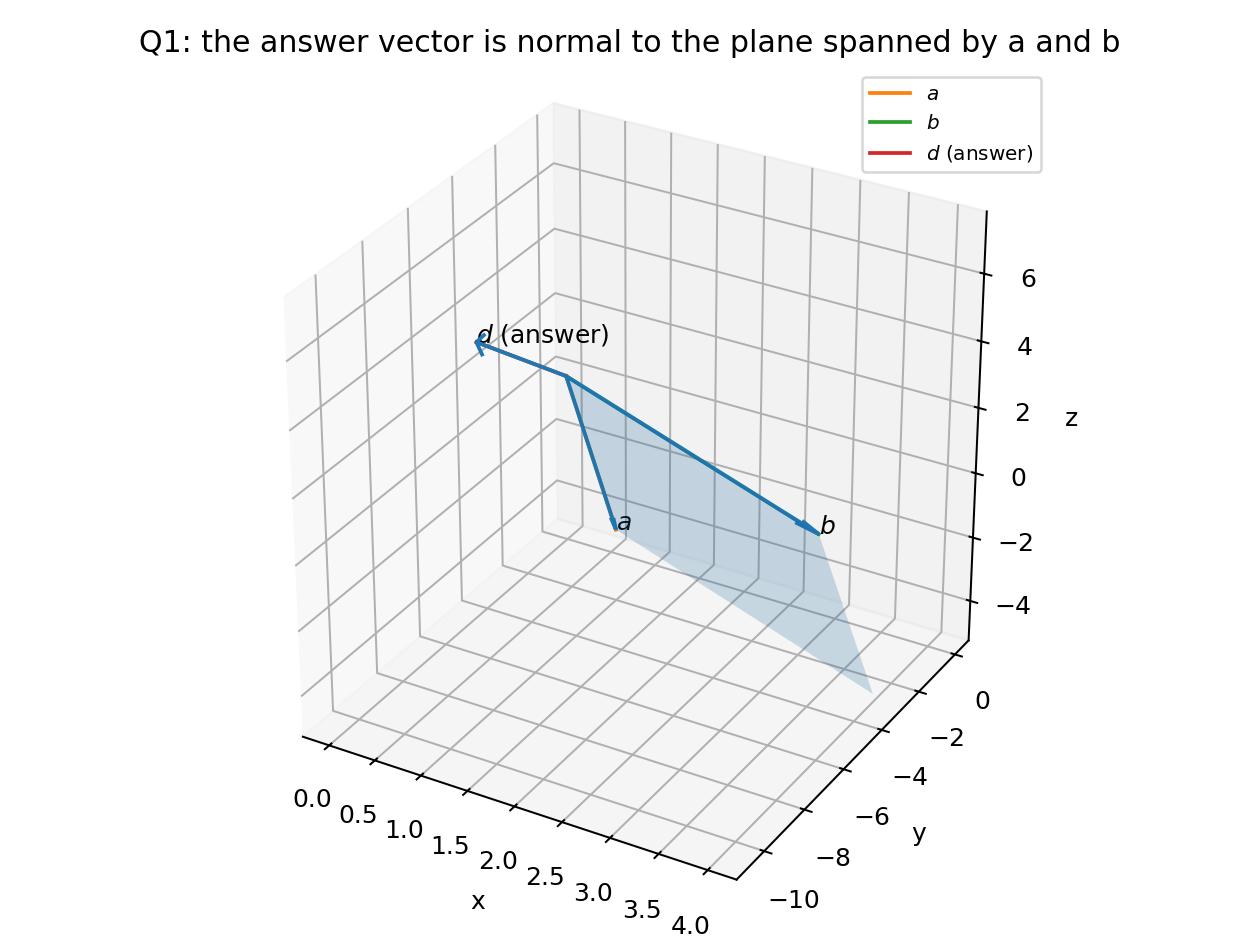
\includegraphics[width=0.96\linewidth]{../CBSE-2015-Class12-Updated-corrected_V3/figs/Q01_3D.png}
\caption{The null-space vector is normal to the span of the two given vectors.}
\end{figure}
\par\smallskip
\noindent\textbf{Code reference -}
\par\noindent\fbox{\parbox{\dimexpr\linewidth-2\fboxsep-2\fboxrule\relax}{\centering
\texttt{../CBSE-2015-Class12-Updated-corrected_V3/codes/Q01.py}}}

\setcounter{enumi}{4}\item Let $\vec a=\myvec{1\\4\\2}$, $\vec b=\myvec{3\\-2\\7}$ and $\vec c=\myvec{2\\-1\\4}$. Find $\vec d$ perpendicular to both $\vec a,\vec b$ with $\vec c\cdot\vec d=27$.
\solution The cross product is an antisymmetric bilinear operation. Its
determinant representation gives
\[
\vec a\times\vec b=
\begin{vmatrix}
\hat i&\hat j&\hat k\\
1&4&2\\
3&-2&7
\end{vmatrix}
=\begin{pmatrix}32\\-1\\-14\end{pmatrix}.
\]
It reverses sign when its inputs are exchanged and is orthogonal to
each input vector. Every vector perpendicular to both is therefore
parallel to this cross product; write
\(\vec d=t(\vec a\times\vec b)\). The scalar constraint is
\[
\vec c\cdot(\vec a\times\vec b)
=(2,-1,4)\cdot(32,-1,-14)=64+1-56=9.
\]
Thus \(9t=27\), so \(t=3\) and the corrected vector is
\[
\boxed{\vec d=(96,-3,-42)^T}.
\]
\begin{figure}[H]\centering
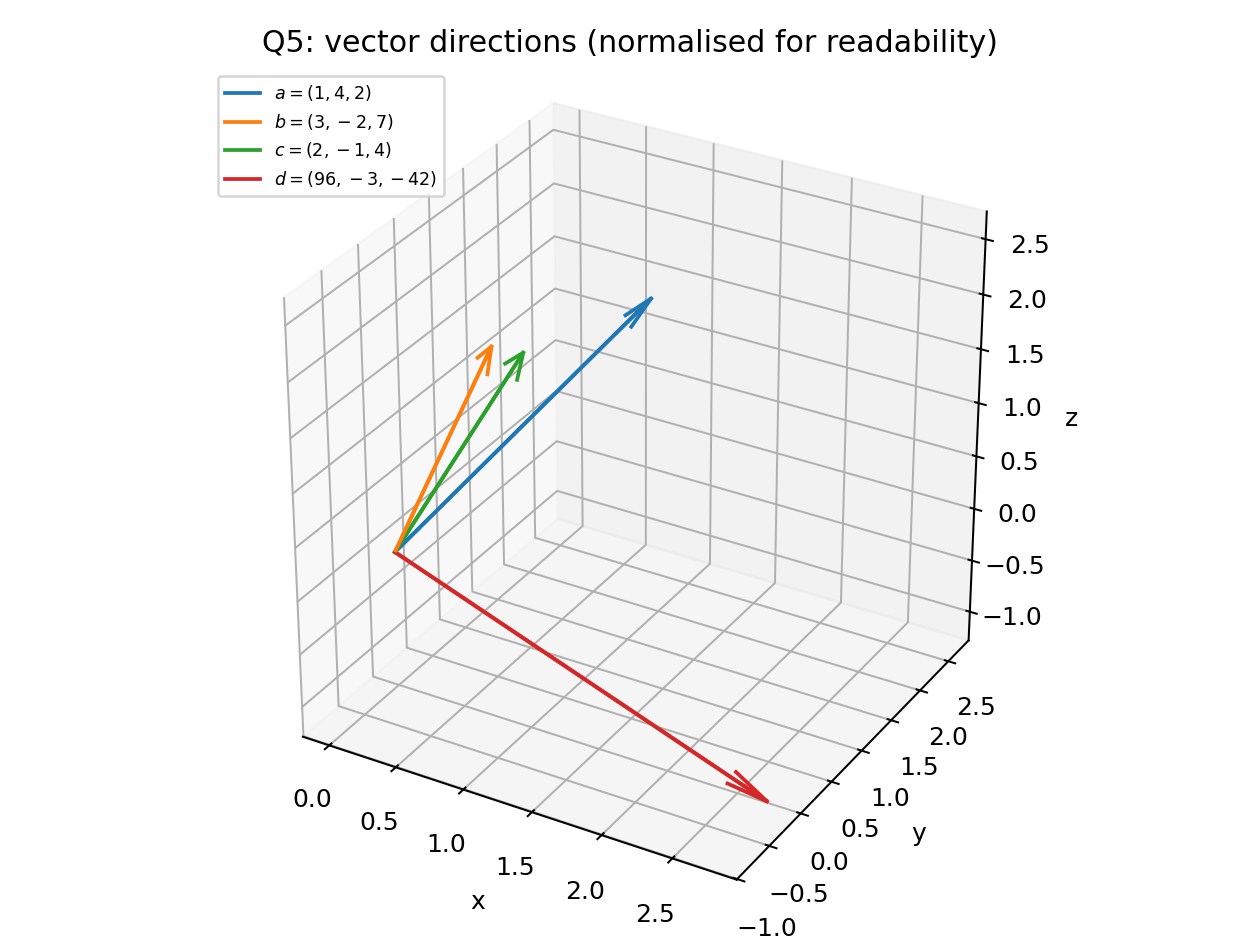
\includegraphics[width=0.96\linewidth]{../CBSE-2015-Class12-Updated-corrected_V3/figs/Q05_3D.png}
\caption{The required vector is normal to both prescribed directions.}
\end{figure}
\par\smallskip
\noindent\textbf{Code reference -}
\par\noindent\fbox{\parbox{\dimexpr\linewidth-2\fboxsep-2\fboxrule\relax}{\centering
\texttt{../CBSE-2015-Class12-Updated-corrected_V3/codes/Q05.py}}}

\setcounter{enumi}{5}\item Find the shortest distance between $\vec r=(1,2,3)+\lambda(2,3,4)$ and $\vec r=(2,4,5)+\mu(4,6,8)$.
\solution The common direction of the parallel lines is \(v=(2,3,4)^T\).
Let \(w=B-A=(1,2,2)^T\). The orthogonal projector onto the line
direction is
\[
P_v=\frac{vv^T}{v^Tv}
=\frac1{29}\begin{pmatrix}
4&6&8\\6&9&12\\8&12&16
\end{pmatrix}.
\]
The parallel component is \(P_vw=(16/29)v\), and the perpendicular
least-squares residual is
\[
r=(I-P_v)w
=\frac1{29}\begin{pmatrix}-3\\10\\-6\end{pmatrix}.
\]
Because \(r^Tv=0\), this is the shortest connector between the lines.
Its norm gives the distance:
\[
d=\|r\|=\frac{\sqrt{145}}{29}
=\boxed{\frac{\sqrt5}{\sqrt{29}}}.
\]
The projection residual makes both the minimizing property and
perpendicularity explicit.
\begin{figure}[H]\centering
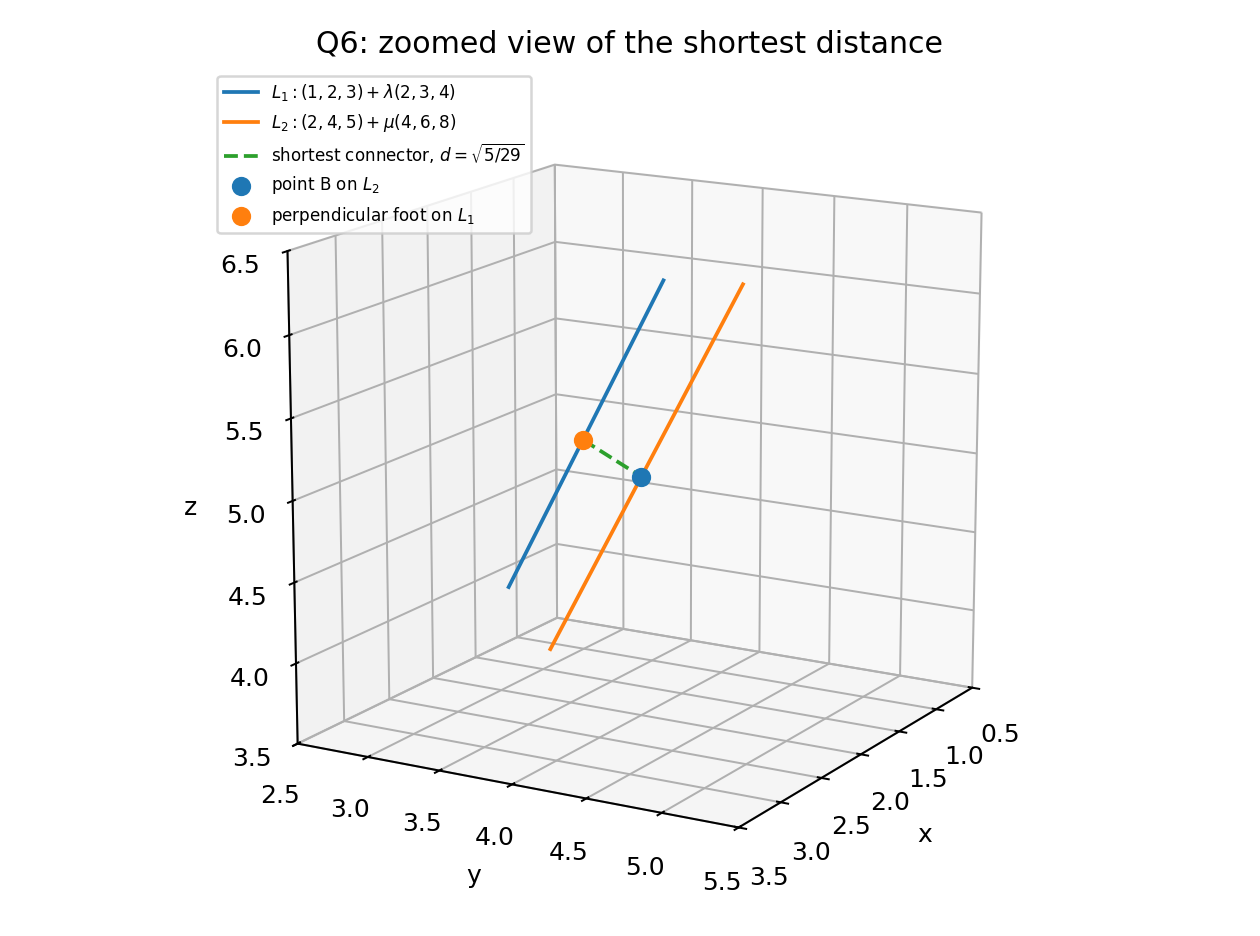
\includegraphics[width=0.96\linewidth]{../CBSE-2015-Class12-Updated-corrected_V3/figs/Q06_3D.png}
\caption{The orthogonal residual joins the closest points on the parallel lines.}
\end{figure}
\par\smallskip
\noindent\textbf{Code reference -}
\par\noindent\fbox{\parbox{\dimexpr\linewidth-2\fboxsep-2\fboxrule\relax}{\centering
\texttt{../CBSE-2015-Class12-Updated-corrected_V3/codes/Q06.py}}}

\paragraph*{Lines and planes}
\setcounter{enumi}{9}\item Find the plane through the intersection of $2x+y-z=3$ and $5x-3y+4z+9=0$ that is parallel to $\frac{x-1}{2}=\frac{y-3}{-4}=\frac{5-z}{-5}$.
\solution Every plane through the intersection of the two specified planes
belongs to their affine plane pencil:
\[
F_1+\lambda F_2=0,\quad
F_1=2x+y-z-3,\quad F_2=5x-3y+4z+9.
\]
Its normal vector is
\[
n(\lambda)=\begin{pmatrix}2+5\lambda\\1-3\lambda\\-1+4\lambda\end{pmatrix}.
\]
The line direction is \(d=(2,-4,5)^T\). For the plane to be parallel
to this line, its normal must satisfy \(n(\lambda)^Td=0\):
\[
2(2+5\lambda)-4(1-3\lambda)+5(-1+4\lambda)=0,
\]
which gives \(42\lambda-5=0\), so \(\lambda=5/42\).
Substitution in the plane pencil yields the corrected plane
\[
\boxed{109x+27y-22z-81=0}.
\]
\begin{figure}[H]\centering
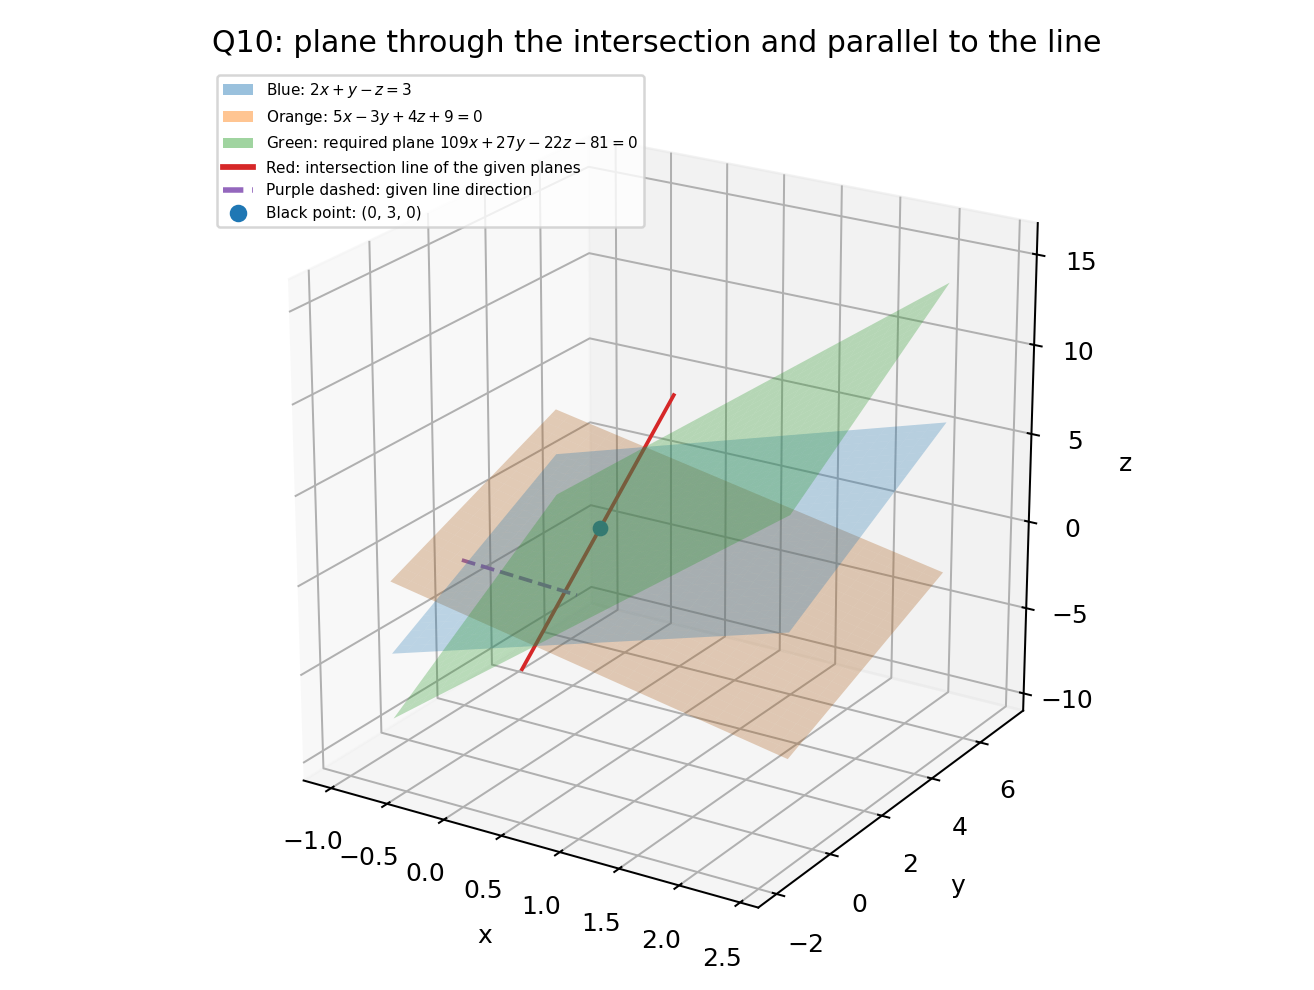
\includegraphics[width=0.96\linewidth]{../CBSE-2015-Class12-Updated-corrected_V3/figs/Q10_3D.png}
\caption{The selected member of the plane pencil is parallel to the given line.}
\end{figure}
\par\smallskip
\noindent\textbf{Code reference -}
\par\noindent\fbox{\parbox{\dimexpr\linewidth-2\fboxsep-2\fboxrule\relax}{\centering
\texttt{../CBSE-2015-Class12-Updated-corrected_V3/codes/Q10.py}}}

\setcounter{enumi}{14}\item Find where the line through $A(3,4,1)$ and $B(5,1,6)$ meets the plane through $P(2,1,2)$, $Q(3,1,0)$ and $R(4,-2,1)$.
\solution The plane through \(P,Q,R\) has normal
\[
(Q-P)\times(R-P)=(1,0,-2)\times(2,-3,-1)=(-6,-3,-3),
\]
so a reduced normal is \(n=(2,1,1)^T\), and the affine plane is
\(2x+y+z=7\). The line \(AB\) has direction \((2,-3,5)^T\).
Formulate the line and plane together as an affine system in
\((x,y,z,t)\):
\[
\begin{pmatrix}
1&0&0&-2\\
0&1&0&3\\
0&0&1&-5\\
2&1&1&0
\end{pmatrix}
\begin{pmatrix}x\\y\\z\\t\end{pmatrix}
=
\begin{pmatrix}3\\4\\1\\7\end{pmatrix}.
\]
The coefficient matrix has rank four, equal to the rank of its
augmented matrix. The system is therefore consistent and has a
unique solution:
\[
t=-\frac23,\qquad
(x,y,z)=\boxed{\left(\frac53,6,-\frac73\right)}.
\]
Substitution into all four affine constraints gives zero residual.
\begin{figure}[H]\centering
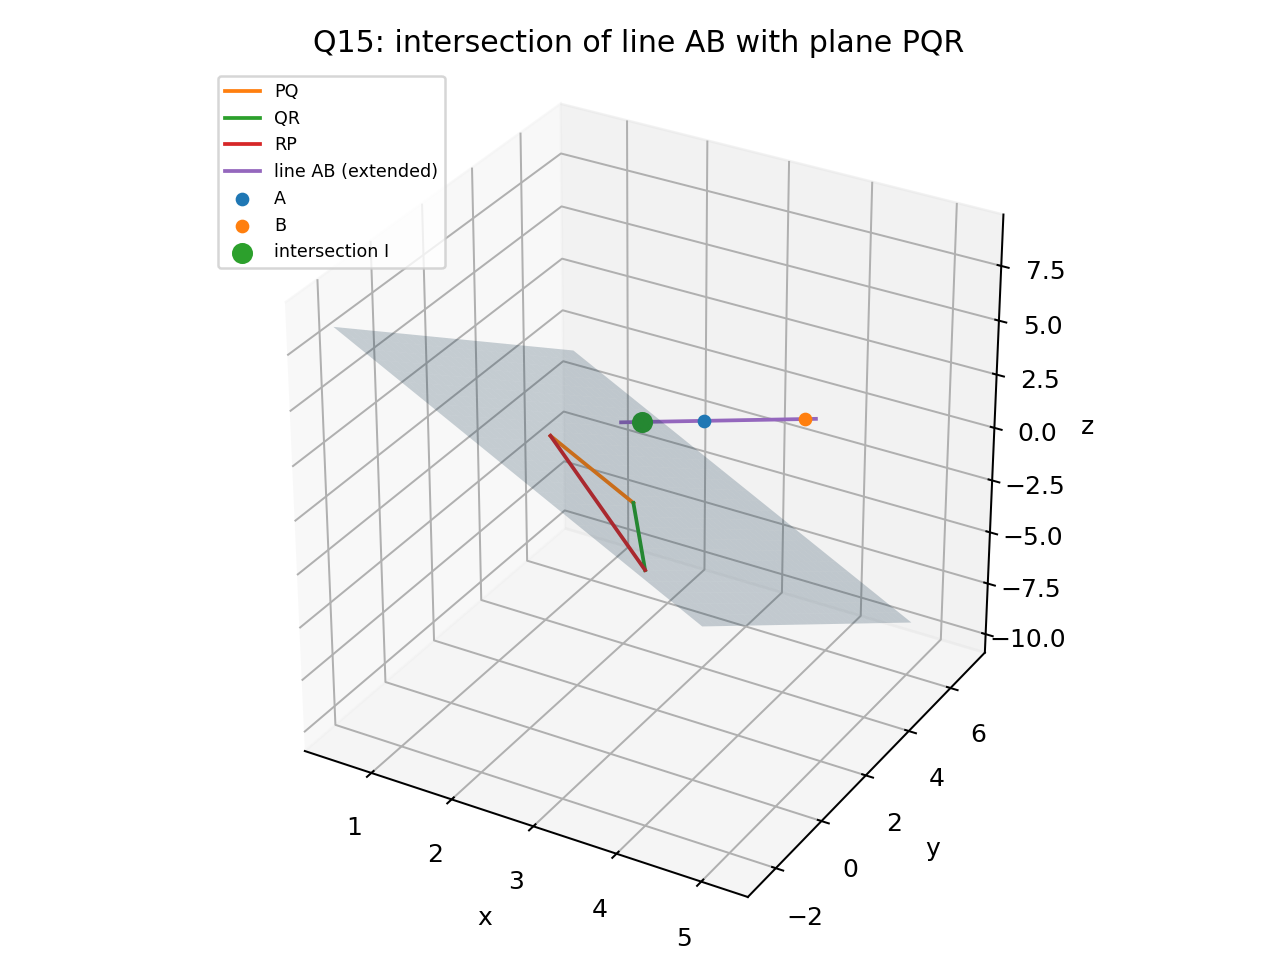
\includegraphics[width=0.96\linewidth]{../CBSE-2015-Class12-Updated-corrected_V3/figs/Q15_3D.png}
\caption{The unique solution of the affine line--plane system.}
\end{figure}
\par\smallskip
\noindent\textbf{Code reference -}
\par\noindent\fbox{\parbox{\dimexpr\linewidth-2\fboxsep-2\fboxrule\relax}{\centering
\texttt{../CBSE-2015-Class12-Updated-corrected_V3/codes/Q15.py}}}

\paragraph*{Differential equations}
\setcounter{enumi}{21}\item Show that $(x-y)\frac{dy}{dx}=x+2y$ is homogeneous and solve it.
\solution Use logarithmic time \(t=\ln|x|\) and the scale-free state
\(u(t)=y(x)/x\), so \(y=xu\) and \(dy/dx=u+du/dt\). Substitution
into the given ODE gives
\[
(1-u)\left(u+\frac{du}{dt}\right)=1+2u,
\]
hence the autonomous dynamical system
\[
\frac{du}{dt}=\frac{1+u+u^2}{1-u},\qquad u\ne1.
\]
The numerator is strictly positive for real \(u\), so the reduced
system has no equilibrium; trajectories are monotone on either side
of the singular state \(u=1\). Separating variables,
\[
\int\frac{1-u}{u^2+u+1}\,du=t+C.
\]
Using
\[
\frac{1-u}{u^2+u+1}
=-\frac12\frac{2u+1}{u^2+u+1}
+\frac32\frac1{u^2+u+1},
\]
integration gives
\[
-\frac12\ln(u^2+u+1)
+\sqrt3\tan^{-1}\!\left(\frac{2u+1}{\sqrt3}\right)
=\ln|x|+C.
\]
Finally substitute \(u=y/x\). The implicit solution holds on
intervals with \(x\ne0\) and does not cross the excluded state \(u=1\).

\setcounter{enumi}{23}\item Find the particular solution of $y'+y\tan x=3x^2+x^3\tan x$, given $y=0$ at $x=\pi/3$ and $x\ne\pi/2$.
\solution Set
\[
u=y-x^3,\qquad \tau=\ln(\sec x).
\]
Then \(y'=u'+3x^2\), and the differential equation reduces to
\(u'+u\tan x=0\). Since \(d\tau/dx=\tan x\), on the branch
containing \(x_0=\pi/3\) this becomes
\[
\frac{du}{d\tau}+u=0.
\]
The initial point gives
\[
\tau_0=\ln2,\qquad
u(\tau_0)=y(\pi/3)-(\pi/3)^3=-\frac{\pi^3}{27}.
\]
Shift to \(\eta=\tau-\tau_0\) and write \(U(\eta)=u(\tau_0+\eta)\).
The unilateral Laplace transform gives
\[
s\bar U(s)-U(0)+\bar U(s)=0,\qquad
\bar U(s)=\frac{-\pi^3/27}{s+1}.
\]
Inverse transformation yields
\[
u=-\frac{\pi^3}{27}e^{-(\tau-\ln2)}
=-\frac{2\pi^3}{27}\cos x,
\]
and therefore
\[
\boxed{y=x^3-\frac{2\pi^3}{27}\cos x}.
\]
The transformed coordinate is monotone on \(0<x<\pi/2\), which
contains the initial point and a neighbourhood on both sides of it.
The displayed solution is regular at \(x=0\) and directly satisfies
the original ODE there, so it extends uniquely across zero to the
maximal interval \(-\pi/2<x<\pi/2\). The endpoints are excluded
because \(\tan x\) is singular there.

\setcounter{enumi}{24}\item If $y=\log\left(\frac{x}{a+bx}\right)^x$, prove that $x^3y''=(xy'-y)^2$.
\solution The question's printed notation is retained:
\(y=\log\left(\frac{x}{a+bx}\right)^x\). The requested identity is
consistent with reading the power as inside the logarithm, namely
\[
y=\log\left[\left(\frac{x}{a+bx}\right)^x\right]
=x\log\left(\frac{x}{a+bx}\right).
\]
Introduce the Euler differential operator \(\theta=x\,d/dx\).
Then
\[
(\theta-1)y=xy'-y=\frac{ax}{a+bx}.
\]
The operator factorization
\[
\theta(\theta-1)y=x^2y''
\]
therefore gives
\[
x^3y''=x\,\theta(\theta-1)y
=x\frac{d}{dx}\left(\frac{ax}{a+bx}\right)
=\frac{a^2x^2}{(a+bx)^2}
=(xy'-y)^2.
\]
This proves the identity wherever the logarithm is defined and
\(a+bx\ne0\). The original question statement is not altered.

\paragraph*{Matrices and determinants}
\setcounter{enumi}{27}\item If $A=\myvec{\cos\theta&\sin\theta\\\sin\theta&\cos\theta}$, find $\det(A^n)$ for natural $n$.
\solution The matrix is real symmetric and has the orthonormal eigenvectors
\[
q_+=\frac1{\sqrt2}\begin{pmatrix}1\\1\end{pmatrix},
\qquad
q_-=\frac1{\sqrt2}\begin{pmatrix}1\\-1\end{pmatrix},
\]
with eigenvalues
\[
\lambda_+=\cos\theta+\sin\theta,\qquad
\lambda_-=\cos\theta-\sin\theta.
\]
Let \(P_\pm=q_\pm q_\pm^T\) be the associated orthogonal spectral
projectors. Then
\[
A=\lambda_+P_++\lambda_-P_-,
\qquad
A^n=\lambda_+^nP_++\lambda_-^nP_-.
\]
The determinant is the product of the eigenvalues, counted with
multiplicity:
\[
\det(A^n)=(\lambda_+\lambda_-)^n
=(\cos^2\theta-\sin^2\theta)^n
=\boxed{(\cos2\theta)^n}.
\]
The orthonormal eigenbasis remains valid even when the eigenvalues
coincide.

\setcounter{enumi}{29}\item Find the inverse of $\myvec{0&1&2\\1&2&3\\3&1&0}$ using elementary row operations.
\solution Let
\[
A=\begin{pmatrix}0&1&2\\1&2&3\\3&1&0\end{pmatrix},
\qquad
P=\begin{pmatrix}0&1&0\\1&0&0\\0&0&1\end{pmatrix}.
\]
The first pivot is obtained by interchanging the first two rows.
An exact factorization is
\[
PA=LU,\quad
L=\begin{pmatrix}1&0&0\\0&1&0\\3&-5&1\end{pmatrix},
\quad
U=\begin{pmatrix}1&2&3\\0&1&2\\0&0&1\end{pmatrix}.
\]
The triangular inverses are
\[
U^{-1}=\begin{pmatrix}1&-2&1\\0&1&-2\\0&0&1\end{pmatrix},
\quad
L^{-1}=\begin{pmatrix}1&0&0\\0&1&0\\-3&5&1\end{pmatrix}.
\]
Since \(PA=LU\), inverse reconstruction gives
\[
A^{-1}=U^{-1}L^{-1}P
=\boxed{\begin{pmatrix}3&-2&1\\-9&6&-2\\5&-3&1\end{pmatrix}}.
\]
The factorization and reconstruction use exact integer arithmetic;
multiplication gives \(AA^{-1}=I_3\).
\par\smallskip
\noindent\textbf{Code reference -}
\par\noindent\fbox{\parbox{\dimexpr\linewidth-2\fboxsep-2\fboxrule\relax}{\centering
\texttt{../CBSE-2015-Class12-Updated-corrected_V3/codes/Q30.py}}}

\setcounter{enumi}{35}\item If $a+b+c\ne0$ and $\mydet{a&b&c\\b&c&a\\c&a&b}=0$, prove that $a=b=c$.
\solution Let
\[
M=\begin{pmatrix}a&b&c\\b&c&a\\c&a&b\end{pmatrix}.
\]
Use the real three-point Fourier basis (the constant DFT mode and
the cosine/sine modes)
\[
q_0=\frac1{\sqrt3}(1,1,1)^T,\quad
q_c=\frac1{\sqrt6}(2,-1,-1)^T,\quad
q_s=\frac1{\sqrt2}(0,1,-1)^T.
\]
For \(Q=(q_0\ q_c\ q_s)\), direct transformation yields
\[
Q^TMQ=
\begin{pmatrix}
a+b+c&0&0\\
0&d&e\\
0&e&-d
\end{pmatrix},
\quad
d=a-\frac{b+c}{2},\qquad e=\frac{\sqrt3}{2}(b-c).
\]
The lower Fourier block has eigenvalues
\[
\lambda_\pm=\pm\sqrt{d^2+e^2}
=\pm\sqrt{a^2+b^2+c^2-ab-bc-ca}.
\]
Thus the full spectrum is \(a+b+c,\lambda_+,\lambda_-\), and
\[
\det M=-(a+b+c)(a^2+b^2+c^2-ab-bc-ca).
\]
The displayed matrix is reverse-circulant, not an ordinary
circulant: the Fourier basis isolates the two-dimensional Fourier
subspace, and that block must then be diagonalized. Since
\(a+b+c\ne0\) and \(\det M=0\), the squared radical is zero. Hence
\[
\frac12\bigl((a-b)^2+(b-c)^2+(c-a)^2\bigr)=0,
\]
which forces
\[
\boxed{a=b=c}.
]

\setcounter{enumi}{36}\item A trust receives Rs. 30,000 per month. Half is spent on care, and 2\% of the amount spent is collected from beneficiaries. The unspent balance is deposited in a bank. Find the monthly interest rate needed for total monthly income of Rs. 1800.
\solution Let $u$ be the monthly contribution collected from beneficiaries and $v$ the bank interest. Half of Rs. $30,000$ is spent, so
\[
u=0.02(15000)=300.
\]
The total monthly income is Rs. $1800$, so
\[
u+v=1800,\qquad u=300.
\]
Write this system as an augmented matrix:
\[
\left[\begin{array}{cc|c}1&1&1800\\1&0&300\end{array}\right]
\xrightarrow{R_2\leftarrow R_2-R_1}
\left[\begin{array}{cc|c}1&1&1800\\0&-1&-1500\end{array}\right]
\xrightarrow{R_2\leftarrow -R_2}
\left[\begin{array}{cc|c}1&1&1800\\0&1&1500\end{array}\right].
\]
Eliminate $v$ from the first row:
\[
R_1\leftarrow R_1-R_2:\qquad
\left[\begin{array}{cc|c}1&0&300\\0&1&1500\end{array}\right]\qquad\eqref{eq:gaussian-elimination}.
\]
Thus $u=300$ and $v=1500$. The deposit is Rs. $15000$, therefore
\[
r=\frac{1500}{15000}\times100\%=10\%\text{ per month}.
\]
\par\smallskip
\noindent\textbf{Code reference -}
\par\noindent\fbox{\parbox{\dimexpr\linewidth-2\fboxsep-2\fboxrule\relax}{\centering\texttt{../CBSE-2015-Class12-Updated-corrected_V3/codes/Q37.py}}}
\par\smallskip



\paragraph*{Integration and area}
\setcounter{enumi}{37}\item Evaluate $\displaystyle I=\int_0^{\pi/2}\frac{\cos^2x}{1+3\sin^2x}\,dx$.
\solution Let $t=\tan x$. Then $dx=dt/(1+t^2)$ and the integral becomes
\[
I=\int_0^\infty\frac{dt}{(1+t^2)(1+4t^2)}=\int_0^\infty\left[-\frac1{3(1+t^2)}+\frac4{3(1+4t^2)}\right]dt.
\]
Evaluating the arctangent limits gives $I=-\pi/6+\pi/3=\pi/6\qquad\eqref{eq:scaled-arctan-integral-38},\ \eqref{eq:arctan-integral-38}$.

\setcounter{enumi}{38}\item Evaluate $\displaystyle\int_0^{\pi/4}\frac{\sin x+\cos x}{3+\sin2x}\,dx$.
\solution Set $u=\sin x-\cos x$, so $du=(\sin x+\cos x)dx$ and $\sin2x=1-u^2$. The limits become $u=-1$ and $u=0$. Hence
\[
I=\int_{-1}^{0}\frac{du}{4-u^2}=\left[\frac14\ln\left|\frac{2+u}{2-u}\right|\right]_{-1}^{0}=\frac14\ln3\qquad\eqref{eq:int-rational-39}.
\]

\setcounter{enumi}{39}\item Evaluate $\displaystyle\int\frac{\sin x-x\cos x}{x(x+\sin x)}\,dx$.
\solution Since
\[
\frac{d}{dx}\ln\left|\frac{x}{x+\sin x}\right|=\frac{\sin x-x\cos x}{x(x+\sin x)}\qquad\eqref{eq:log-derivative-40},
\]
the integral is $\ln\left|\frac{x}{x+\sin x}\right|+C$.

\setcounter{enumi}{40}\item Evaluate $\displaystyle\int\frac{x^3}{(x-1)(x^2+1)}\,dx$.
\solution Polynomial division and partial fractions give
\[
\frac{x^3}{(x-1)(x^2+1)}=1+\frac1{2(x-1)}+\frac{x-1}{2(x^2+1)}\qquad\eqref{eq:partial-fractions-41}.
\]
Therefore
\[
x+\frac12\ln|x-1|+\frac14\ln(x^2+1)-\frac12\tan^{-1}x+C.
\]

\setcounter{enumi}{41}\item Find $\displaystyle\int\frac{x\,dx}{1+x\tan x}$.
\solution Rewrite the integrand as $x\cos x/(\cos x+x\sin x)$. Since $d(\cos x+x\sin x)/dx=x\cos x$,
\[
\int\frac{x\,dx}{1+x\tan x}=\ln|\cos x+x\sin x|+C\qquad\eqref{eq:log-derivative-42}.
\]

\setcounter{enumi}{42}\item Evaluate $\displaystyle\int\frac{x^4}{(x-1)(x^2+1)}\,dx$.
\solution Division gives $x^4/[(x-1)(x^2+1)]=x+1+1/[(x-1)(x^2+1)]$. Decompose the last term as
\[
\frac1{(x-1)(x^2+1)}=\frac1{2(x-1)}-\frac{x+1}{2(x^2+1)}\qquad\eqref{eq:partial-fractions-43}.
\]
Thus
\[
\frac{x^2}{2}+x+\frac12\ln|x-1|-\frac14\ln(x^2+1)-\frac12\tan^{-1}x+C.
\]

\setcounter{enumi}{43}\item Evaluate $\displaystyle\int_0^{\pi/2}\frac{5\sin x+3\cos x}{\sin x+\cos x}\,dx$.
\solution Write the numerator as $4(\sin x+\cos x)+(\sin x-\cos x)$. Then
\[
I=4\int_0^{\pi/2}dx-\left[\ln(\sin x+\cos x)\right]_0^{\pi/2}=2\pi\qquad\eqref{eq:trig-split-44}.
\]

\setcounter{enumi}{44}\item Find $\displaystyle\int\left[\log(\log x)+\frac1{(\log x)^2}\right]dx$.
\solution Differentiate $x\log(\log x)-x/\log x$ to check that it equals the integrand. Hence
\[
x\log(\log x)-\frac{x}{\log x}+C,\qquad x>1\text{ for a real-valued }\log(\log x).
\]

\setcounter{enumi}{45}\item If the area bounded by $y^2=16ax$ and $y=4mx$ is $a^2/2$, find $m$.
\solution Use the upper branch $y=4\sqrt{ax}$. At an intersection with $y=4mx$,
\[
4\sqrt{ax}=4mx\quad\Longrightarrow\quad x=0\quad\text{or}\quad x=\frac{a}{m^2}.
\]
For positive slope, the area is the integral of the parabola minus the line:
\begin{align*}
A&=\int_0^{a/m^2}\left(4\sqrt{ax}-4mx\right)\,dx\\
 &=\left[\frac{8\sqrt a}{3}x^{3/2}-2mx^2\right]_0^{a/m^2}\\
 &=\frac{8a^2}{3m^3}-\frac{2a^2}{m^3}=\frac{2a^2}{3m^3}\qquad\eqref{eq:area-between-46}.
\end{align*}
Set the result equal to the given area:
\[
\frac{2a^2}{3m^3}=\frac{a^2}{2}\quad\Longrightarrow\quad4=3m^3\quad\Longrightarrow\quad m=\sqrt[3]{\frac43}.
\]
The graph uses $a=1$ for visibility; the value of $m$ is independent of that scale.
\begin{figure}[H]\centering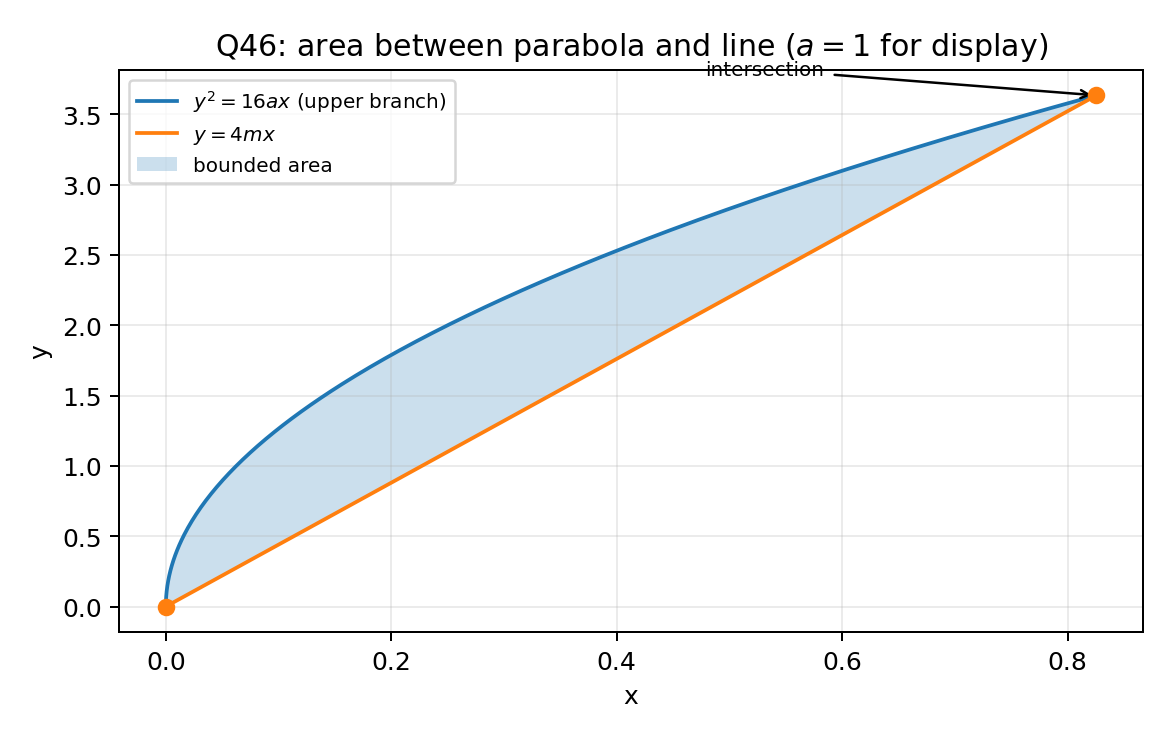
\includegraphics[width=0.92\linewidth]{../CBSE-2015-Class12-Updated-corrected_V3/figs/Q46_ParabolaArea.png}\end{figure}
\par\smallskip
\noindent\textbf{Code reference -}
\par\noindent\fbox{\parbox{\dimexpr\linewidth-2\fboxsep-2\fboxrule\relax}{\centering\texttt{../CBSE-2015-Class12-Updated-corrected_V3/codes/Q46.py}}}
\par\smallskip

\setcounter{enumi}{46}\item Find the area of $\{(x,y):x^2+y^2\le4,\;x+y\ge2\}$ by integration.
\solution The chord $x+y=2$ meets the circle at $(0,2)$ and $(2,0)$. For $0\le x\le2$, the upper circle boundary is $y=\sqrt{4-x^2}$ and the line is $y=2-x$. Therefore
\begin{align*}
A&=\int_0^2\left(\sqrt{4-x^2}-(2-x)\right)dx\\
 &=\underbrace{\int_0^2\sqrt{4-x^2}\,dx}_{\text{quarter-circle area }=\pi}
 -\underbrace{\int_0^2(2-x)\,dx}_{\text{triangle area }=2}\\
 &=\pi-2\quad\text{square units}\qquad\eqref{eq:area-between-47}.
\end{align*}
The graph shades the circular segment above the chord.
\begin{figure}[H]\centering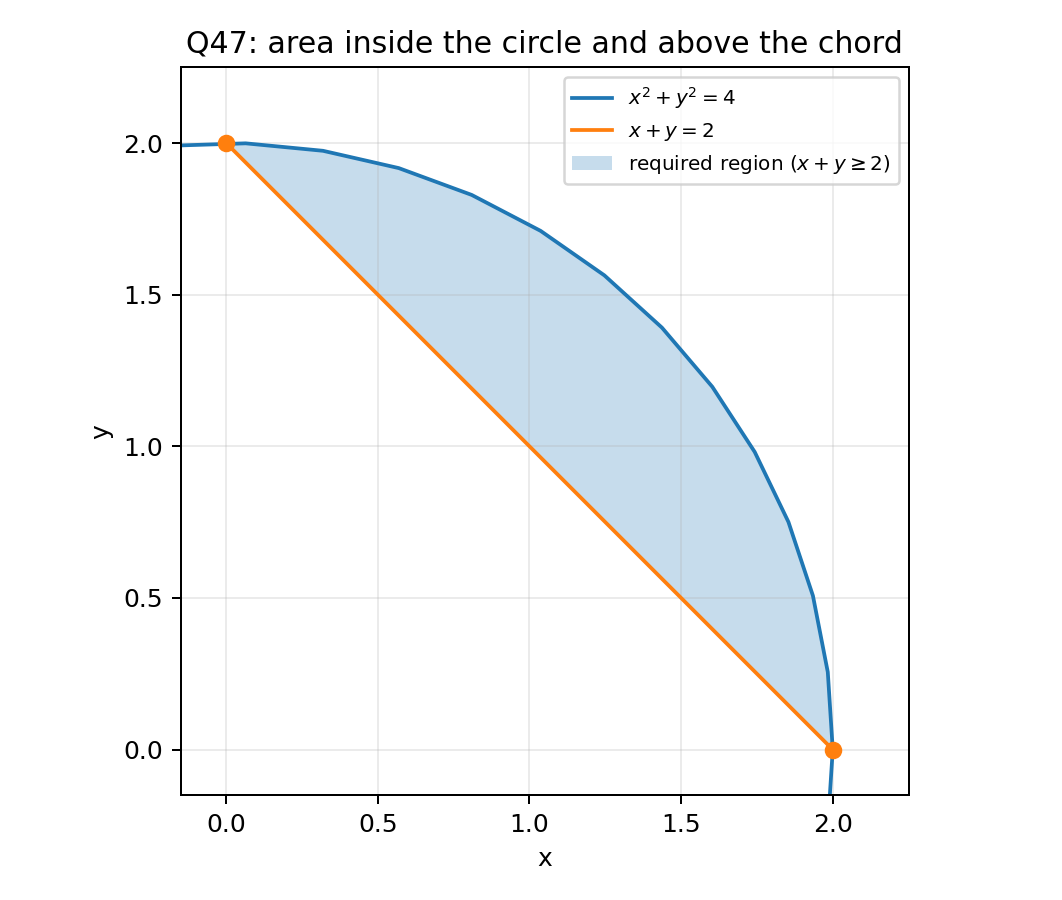
\includegraphics[width=0.92\linewidth]{../CBSE-2015-Class12-Updated-corrected_V3/figs/Q47_CircleSegment.png}\end{figure}
\par\smallskip
\noindent\textbf{Code reference -}
\par\noindent\fbox{\parbox{\dimexpr\linewidth-2\fboxsep-2\fboxrule\relax}{\centering\texttt{../CBSE-2015-Class12-Updated-corrected_V3/codes/Q47.py}}}
\par\smallskip


\paragraph*{Functions and relations}
\setcounter{enumi}{47}\item Discuss continuity and differentiability of $f(x)=|x|+|x-1|$ on $(-1,2)$.
\solution First split the absolute values at $x=0$ and $x=1$:
\[
f(x)=\begin{cases}
1-2x,&-1<x<0,\\
1,&0\le x<1,\\
2x-1,&1\le x<2.
\end{cases}
\]
\textbf{Continuity.} At $x=0$, the left limit, right limit and function value are all $1$. The same is true at $x=1$. Each branch is continuous on its interval; hence $f$ is continuous throughout $(-1,2)$.

\textbf{Differentiability at $x=0$.} The left-hand slope is $-2$ and the right-hand slope is $0$:
\[
f'_-(0)=-2\ne0=f'_+(0).
\]
Thus $f$ is not differentiable at $0$.

\textbf{Differentiability at $x=1$.} The left-hand slope is $0$ and the right-hand slope is $2$ (see the one-sided derivative criterion \eqref{eq:continuity-differentiability-48}):
\[
f'_-(1)=0\ne2=f'_+(1).
\]
Thus $f$ is not differentiable at $1$. At other points the function is linear and differentiable. The plot shows these one-sided slopes: differentiability requires equal one-sided slopes, and the two corners fail that test.
\begin{figure}[H]\centering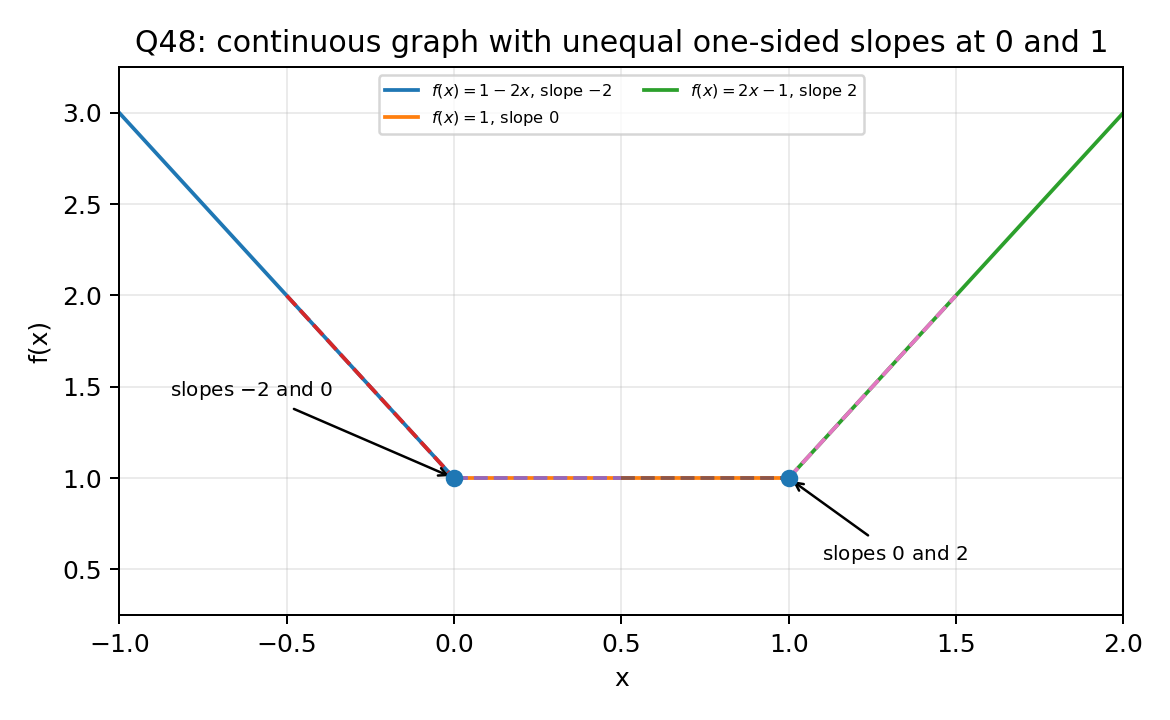
\includegraphics[width=0.92\linewidth]{../CBSE-2015-Class12-Updated-corrected_V3/figs/Q48_Differentiability.png}\end{figure}
\par\smallskip
\noindent\textbf{Code reference -}
\par\noindent\fbox{\parbox{\dimexpr\linewidth-2\fboxsep-2\fboxrule\relax}{\centering\texttt{../CBSE-2015-Class12-Updated-corrected_V3/codes/Q48.py}}}
\par\smallskip

\setcounter{enumi}{48}\item On $\mathbb R$, define $(a,b)\in R$ when $a-b+\sqrt3$ is irrational. Determine whether $R$ is reflexive, symmetric and transitive.
\solution We test each property separately using the criteria in \eqref{eq:relation-properties-49}.

\textbf{1. Reflexive.} Reflexivity requires $(a,a)\in R$ for every real $a$. Substituting $b=a$ gives
\[
a-a+\sqrt3=\sqrt3,
\]
which is irrational. Therefore $R$ is reflexive.

\textbf{2. Symmetric.} Symmetry requires $(a,b)\in R$ to imply $(b,a)\in R$. Choose $a=\sqrt3$ and $b=0$. Then
\[
a-b+\sqrt3=2\sqrt3
\]
is irrational, so $(a,b)\in R$. Reversing the pair gives
\[
b-a+\sqrt3=0,
\]
which is rational, so $(b,a)\notin R$. Hence $R$ is not symmetric.

\textbf{3. Transitive.} Transitivity requires $(a,b),(b,c)\in R$ to imply $(a,c)\in R$. Choose $a=\sqrt3$, $b=0$, and $c=2\sqrt3$. Then
\[
a-b+\sqrt3=2\sqrt3,\qquad b-c+\sqrt3=-\sqrt3,
\]
both irrational, so $(a,b),(b,c)\in R$. However,
\[
a-c+\sqrt3=\sqrt3-2\sqrt3+\sqrt3=0,
\]
which is rational. Thus $(a,c)\notin R$, and $R$ is not transitive.

\textbf{Conclusion.} $R\text{ is reflexive, but neither symmetric nor transitive.}$

\setcounter{enumi}{49}\item On $\mathbb R\times\mathbb R$, define $(a,b)*(c,d)=(a+c,b+d)$. Prove commutativity and associativity, and find the identity and the inverse of $(3,-5)$.
\solution Addition of real components is commutative and associative, so $*$ has both properties. Its identity is $(0,0)$, since $(a,b)*(0,0)=(a,b)$. The inverse of $(3,-5)$ is $(-3,5)$\qquad\eqref{eq:componentwise-operation-50}.

\setcounter{enumi}{50}\item On $\{0,1,2,3,4,5,6\}$ define $a*b=a+b$ if $a+b<7$, and $a*b=a+b-7$ otherwise. Give the operation table and show that 0 is the identity and $7-a$ is the inverse for nonzero $a$.
\solution This is addition modulo 7 \eqref{eq:modular-operation-51}. Its table is
\[
\begin{array}{c|rrrrrrr}
* &0&1&2&3&4&5&6\\\hline
0&0&1&2&3&4&5&6\\
1&1&2&3&4&5&6&0\\
2&2&3&4&5&6&0&1\\
3&3&4&5&6&0&1&2\\
4&4&5&6&0&1&2&3\\
5&5&6&0&1&2&3&4\\
6&6&0&1&2&3&4&5
\end{array}
\]
Row and column 0 reproduce every element, hence 0 is the identity. For each $a=1,\ldots,6$, $a+(7-a)=7\equiv0\pmod7$, so $7-a$ is its inverse.

\setcounter{enumi}{51}\item Find any point of discontinuity of $f(x)=x-|x-x^2|$, $x\in[-1,1]$.
\solution On $[-1,1]$, $x-x^2=x(1-x)$, whose sign changes only at 0. Thus
\[
f(x)=\begin{cases}2x-x^2,&-1\le x\le0,\\x^2,&0\le x\le1.\end{cases}
\]
Both pieces take value 0 at $x=0$ and meet continuously \eqref{eq:continuity-limits-52}. The endpoints are also included continuously. Therefore there are \text{no points of discontinuity}.
\begin{figure}[H]\centering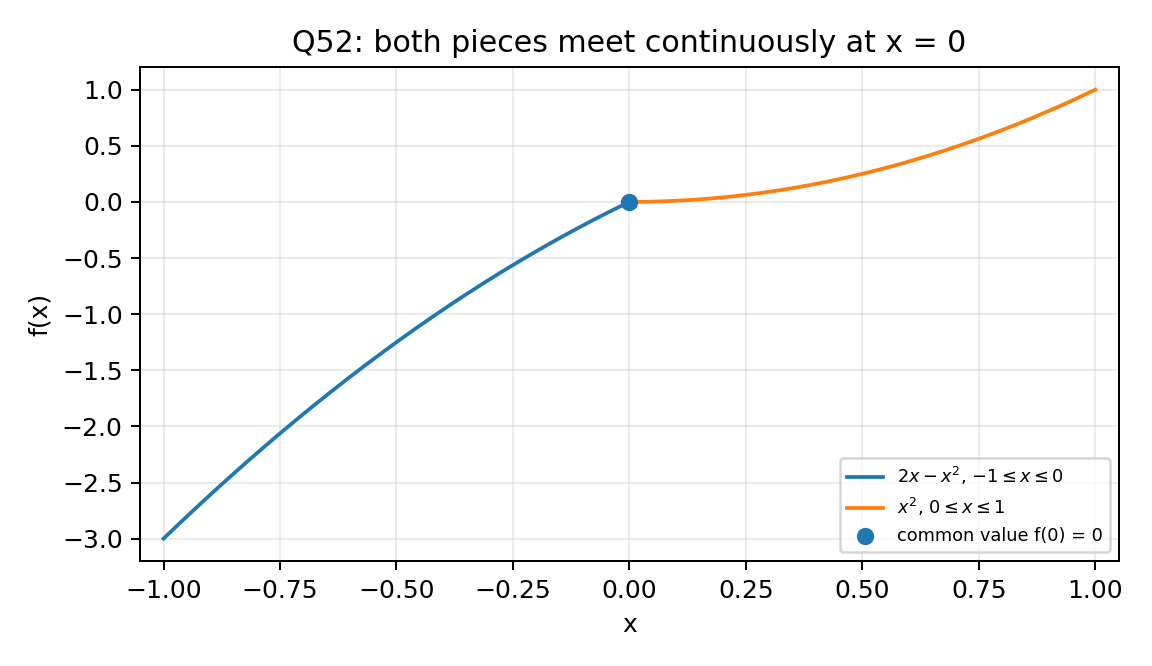
\includegraphics[width=0.92\linewidth]{../CBSE-2015-Class12-Updated-corrected_V3/figs/Q52_Continuity.png}\end{figure}
\par\smallskip
\noindent\textbf{Code reference -}
\par\noindent\fbox{\parbox{\dimexpr\linewidth-2\fboxsep-2\fboxrule\relax}{\centering\texttt{../CBSE-2015-Class12-Updated-corrected_V3/codes/Q52.py}}}
\par\smallskip


\paragraph*{Probability}
\setcounter{enumi}{52}\item A man steps forward with probability $0.4$ and backward with probability $0.6$. Find the probability that after 5 steps he is one step away from his starting point.
\solution Let $k$ be the number of forward steps. The net displacement after five steps is
\[
D=k-(5-k)=2k-5.
\]
One step away means $D=+1$ or $D=-1$. These occur when $k=3$ or $k=2$, respectively.

\textbf{Step 1: Net displacement $+1$.} Three steps are forward and two backward, so the binomial formula gives
\begin{align*}
P(D=1)&=\binom53(0.4)^3(0.6)^2\\
&=10(0.064)(0.36)=0.2304\qquad\eqref{eq:binomial-53}.
\end{align*}

\textbf{Step 2: Net displacement $-1$.} Two steps are forward and three backward:
\begin{align*}
P(D=-1)&=\binom52(0.4)^2(0.6)^3\\
&=10(0.16)(0.216)=0.3456.
\end{align*}

\textbf{Step 3: Add the disjoint events.}
\[
P(|D|=1)=P(D=1)+P(D=-1)=0.2304+0.3456=0.576.
\]

\textbf{Generating function / $Z$-transform.} For one step, the Laurent probability generating function is $G(z)=0.4z+0.6z^{-1}$. For five independent steps,
\[
G_5(z)=(0.4z+0.6z^{-1})^5
=\sum_{k=0}^5\binom5k(0.4)^k(0.6)^{5-k}z^{2k-5}\qquad\eqref{eq:walk-pgf}.
\]
The coefficient of $z^1$ is $0.2304$ and the coefficient of $z^{-1}$ is $0.3456$. Their sum is the required probability. The plot shows the theoretical PMF for every possible displacement.
\begin{figure}[H]\centering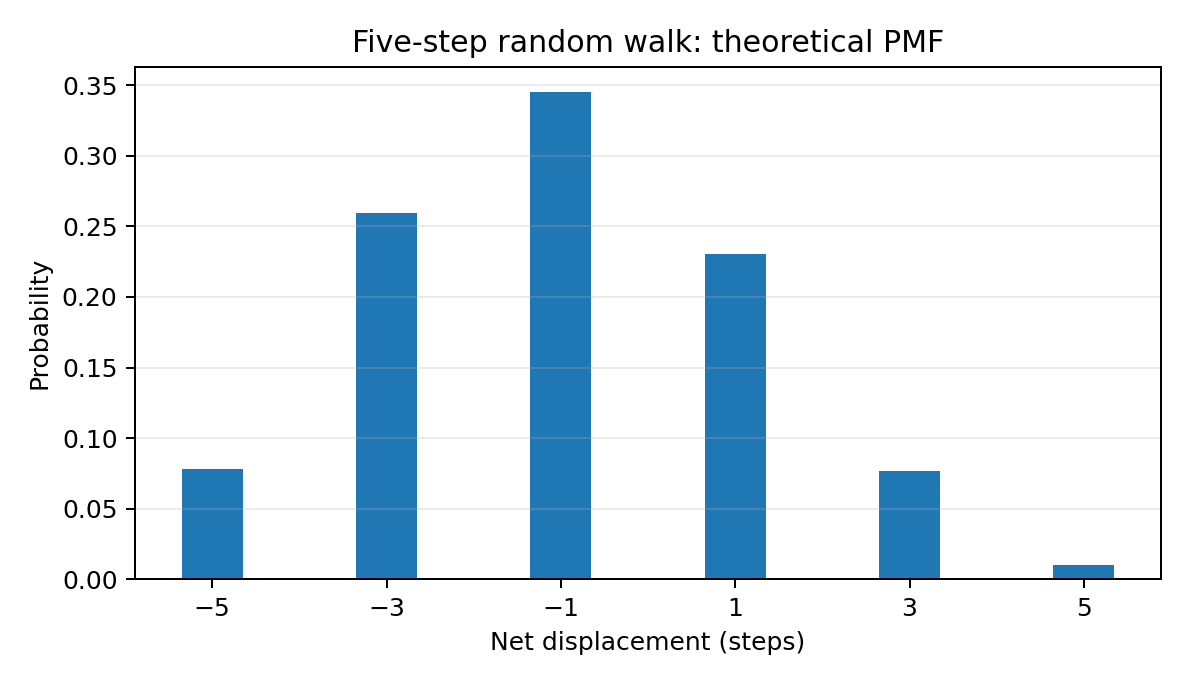
\includegraphics[width=0.92\linewidth]{../CBSE-2015-Class12-Updated-corrected_V3/figs/Q53_WalkPMF.png}\end{figure}
\par\smallskip
\noindent\textbf{Code reference -}
\par\noindent\fbox{\parbox{\dimexpr\linewidth-2\fboxsep-2\fboxrule\relax}{\centering\texttt{../CBSE-2015-Class12-Updated-corrected_V3/codes/Q53.py}}}
\par\smallskip

\setcounter{enumi}{53}\item A girl throws a die. If it shows 1 or 2, she tosses a coin three times; otherwise she tosses it once. Given that exactly one tail was obtained, find the probability that the die showed 3, 4, 5 or 6.
\solution Let $A$ mean that the die shows 1 or 2, $B$ mean that it shows 3, 4, 5 or 6, and $E$ mean that exactly one tail is observed.

\textbf{Step 1: Find the prior probabilities.}
\[
P(A)=\frac26=\frac13,\qquad P(B)=\frac46=\frac23.
\]

\textbf{Step 2: Find the likelihood of $E$.} If $A$ occurs, three fair coin tosses are made. Exactly one tail can occur in $\binom31$ of the 8 equally likely outcomes:
\[
P(E\mid A)=\binom31\left(\frac12\right)^3=\frac38.
\]
If $B$ occurs, only one coin toss is made, so
\[
P(E\mid B)=\frac12.
\]

\textbf{Step 3: Calculate $P(E)$ by total probability.}
\begin{align*}
P(E)&=P(E\mid A)P(A)+P(E\mid B)P(B)\\
&=\frac38\cdot\frac13+\frac12\cdot\frac23\\
&=\frac18+\frac13=\frac{11}{24}\qquad\eqref{eq:total-probability-54}.
\end{align*}

\textbf{Step 4: Apply Bayes' theorem.}
\[
P(B\mid E)=\frac{P(E\mid B)P(B)}{P(E)}
=\frac{(1/2)(2/3)}{11/24}=\frac8{11}\qquad\eqref{eq:bayes-54}.
\]

\setcounter{enumi}{54}\item An urn contains 5 red and 2 black balls. Two balls are drawn without replacement. Let $X$ be the number of black balls. State its possible values and find its mean and variance.
\solution The possible values are $0,1,2$. The probabilities from the hypergeometric model are
\[
P(X=0)=\frac{10}{21},\quad P(X=1)=\frac{10}{21},\quad P(X=2)=\frac1{21}\qquad\eqref{eq:hypergeometric-55}.
\]
So $E[X]=0(10/21)+1(10/21)+2(1/21)=4/7$. Also $E[X^2]=10/21+4/21=2/3$, hence
\[
\operatorname{Var}(X)=E[X^2]-E[X]^2=\frac23-\frac{16}{49}=\frac{50}{147}\qquad\eqref{eq:mean-variance-55}.
\]
\begin{figure}[H]\centering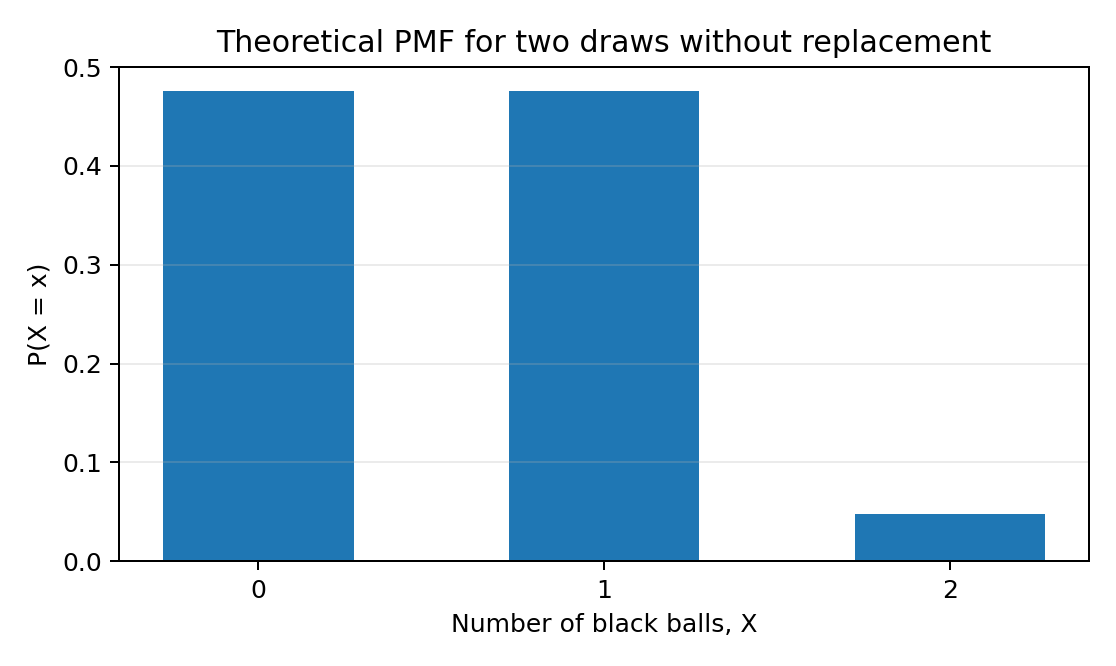
\includegraphics[width=0.90\linewidth]{../CBSE-2015-Class12-Updated-corrected_V3/figs/Q55_BlackBallsPMF.png}\end{figure}
\par\smallskip
\noindent\textbf{Code reference -}
\par\noindent\fbox{\parbox{\dimexpr\linewidth-2\fboxsep-2\fboxrule\relax}{\centering\texttt{../CBSE-2015-Class12-Updated-corrected_V3/codes/Q55.py}}}
\par\smallskip

\setcounter{enumi}{55}\item In 3 trials of a binomial distribution, the probability of exactly 2 successes is 9 times the probability of 3 successes. Find the success probability.
\solution Let the success probability be $p$ and $q=1-p$. The probability-generating polynomial is
\[
B(z)=(q+pz)^3=q^3+3pq^2z+3p^2qz^2+p^3z^3.
\]
The coefficient of $z^2$ is
\[
P(X=2)=\binom32p^2q=3p^2q\qquad\eqref{eq:binomial-56},
\]
and the coefficient of $z^3$ is
\[
P(X=3)=p^3.
\]
Use $P(X=2)=9P(X=3)$:
\begin{align*}
3p^2q&=9p^3,\\
3p^2(1-p)&=9p^3.
\end{align*}
For the non-degenerate binomial case $p>0$, divide by $3p^2$: $1-p=3p$. Thus $4p=1$ and
\[
p=\frac14.
\]
The polynomial's coefficients directly identify the two probabilities; no separate $Z$-transform is needed beyond this generating-polynomial viewpoint.
\par\smallskip
\noindent\textbf{Code reference -}
\par\noindent\fbox{\parbox{\dimexpr\linewidth-2\fboxsep-2\fboxrule\relax}{\centering\texttt{../CBSE-2015-Class12-Updated-corrected_V3/codes/Q56.py}}}
\par\smallskip

\setcounter{enumi}{56}\item An urn contains 3 red and 5 black balls. A ball is drawn, its colour recorded and returned, and 2 more balls of that colour are added. Then two balls are drawn without replacement. Find the probability both are red.
\solution If the first ball is red, with probability $3/8$, the urn becomes 5 red and 5 black; the chance of two reds is $(5/10)(4/9)=2/9$. If the first ball is black, with probability $5/8$, the urn becomes 3 red and 7 black; the chance of two reds is $(3/10)(2/9)=1/15$. Thus
\[
P(\text{two red})=\frac38\frac29+\frac58\frac1{15}=\frac18\qquad\eqref{eq:total-probability-57}.
\]
\par\smallskip
\noindent\textbf{Code reference -}
\par\noindent\fbox{\parbox{\dimexpr\linewidth-2\fboxsep-2\fboxrule\relax}{\centering\texttt{../CBSE-2015-Class12-Updated-corrected_V3/codes/Q57.py}}}
\par\smallskip

\paragraph*{Linear programming}
\setcounter{enumi}{58}\item Solve graphically: minimise $z=3x+5y$ subject to $x+2y\ge10$, $x+y\ge6$, $3x+y\ge8$, $x,y\ge0$.
\solution The lower-boundary vertices are $(0,8)$, $(1,5)$, $(2,4)$ and $(10,0)$. Their objective values are respectively $40$, $28$, $26$ and $30$. The smallest value is attained at $(2,4)$:
\[
x=2,\ y=4,\ z_{\min}=26\qquad\eqref{eq:lpp-59}.
\]
\begin{figure}[H]\centering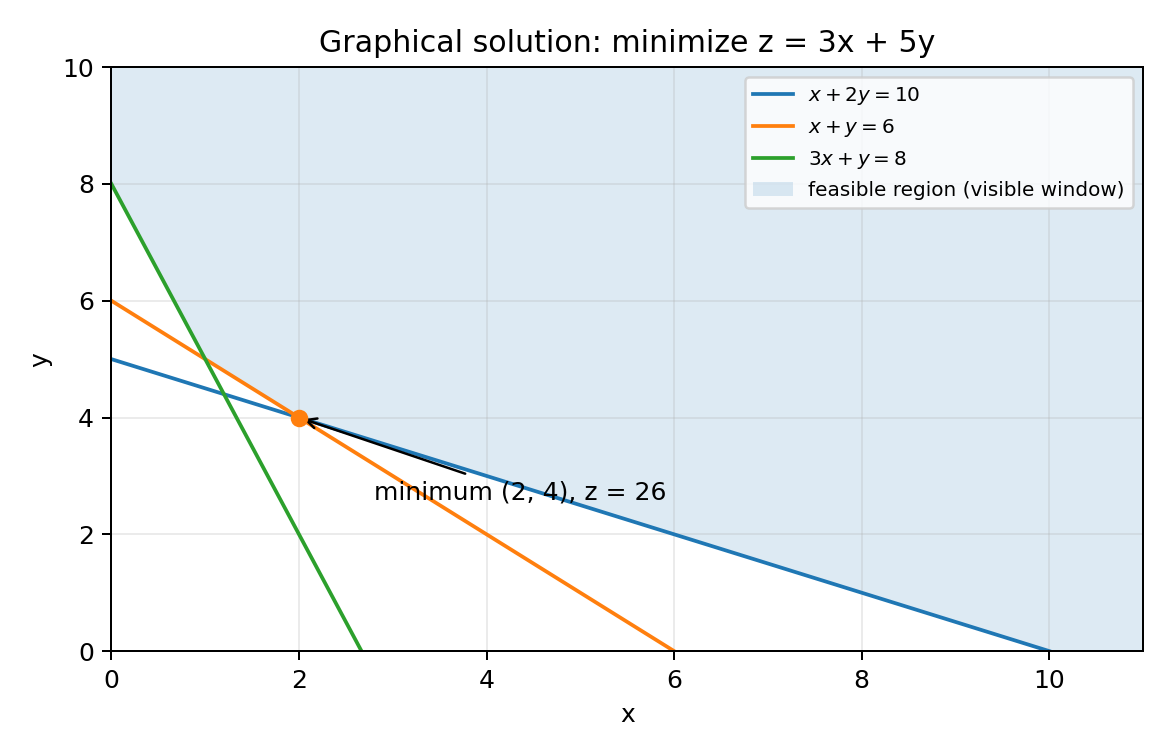
\includegraphics[width=0.92\linewidth]{../CBSE-2015-Class12-Updated-corrected_V3/figs/Q59_LPPMin.png}\end{figure}
\par\smallskip
\noindent\textbf{Code reference -}
\par\noindent\fbox{\parbox{\dimexpr\linewidth-2\fboxsep-2\fboxrule\relax}{\centering\texttt{../CBSE-2015-Class12-Updated-corrected_V3/codes/Q59.py}}}
\par\smallskip

\setcounter{enumi}{59}\item A dealer has Rs. 57,600 and space for at most 20 sewing machines. An electronic machine costs Rs. 3600 and earns Rs. 220 profit; a manual machine costs Rs. 2400 and earns Rs. 180 profit. How should he invest to maximise profit?
\solution Let $x$ and $y$ be electronic and manual machines. The constraints are $3x+2y\le48$, $x+y\le20$, $x,y\ge0$, and profit is $P=220x+180y$. At the intersection of the two active limits, $3x+2y=48$ and $x+y=20$, we get $(x,y)=(8,12)$ and $P=3920$. The axis vertices give profits Rs. 3520 and Rs. 3600. Therefore the best feasible integer plan is
\[
8\text{ electronic and }12\text{ manual machines; maximum profit Rs. }3920\qquad\eqref{eq:lpp-60}.
\]
\begin{figure}[H]\centering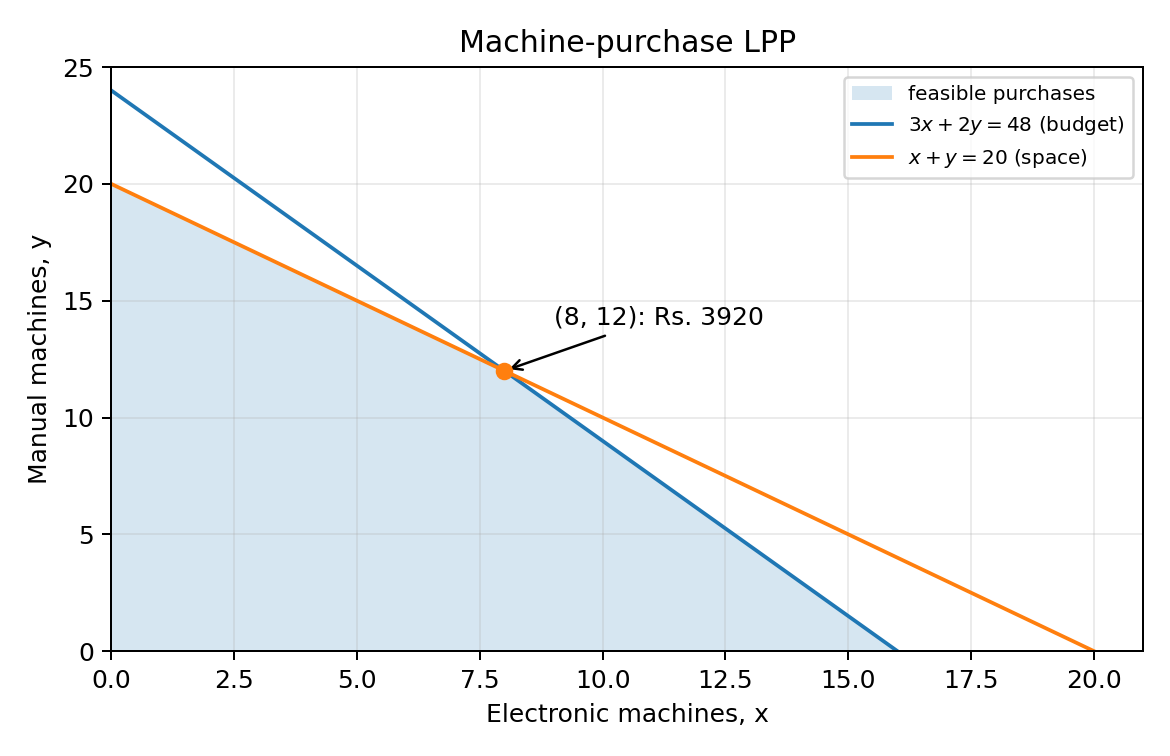
\includegraphics[width=0.92\linewidth]{../CBSE-2015-Class12-Updated-corrected_V3/figs/Q60_LPPProfit.png}\end{figure}
\par\smallskip
\noindent\textbf{Code reference -}
\par\noindent\fbox{\parbox{\dimexpr\linewidth-2\fboxsep-2\fboxrule\relax}{\centering\texttt{../CBSE-2015-Class12-Updated-corrected_V3/codes/Q60.py}}}
\par\smallskip




\paragraph*{Coordinate geometry and optimisation}
\setcounter{enumi}{63}\item A tangent to $x^2+y^2=4$ at a point in the first quadrant meets the positive axes at $A$ and $B$. Find the minimum of $OA+OB$.
\solution At the point $(2\cos\theta,2\sin\theta)$, the tangent is $x\cos\theta+y\sin\theta=2$. Thus $OA=2\sec\theta$ and $OB=2\csc\theta$. By symmetry (or differentiating), their sum is minimised when $\sin\theta=\cos\theta=1/\sqrt2$. Hence
\[
\min(OA+OB)=2(\sqrt2+\sqrt2)=4\sqrt2\qquad\eqref{eq:circle-tangent-64}.
\]
\begin{figure}[H]\centering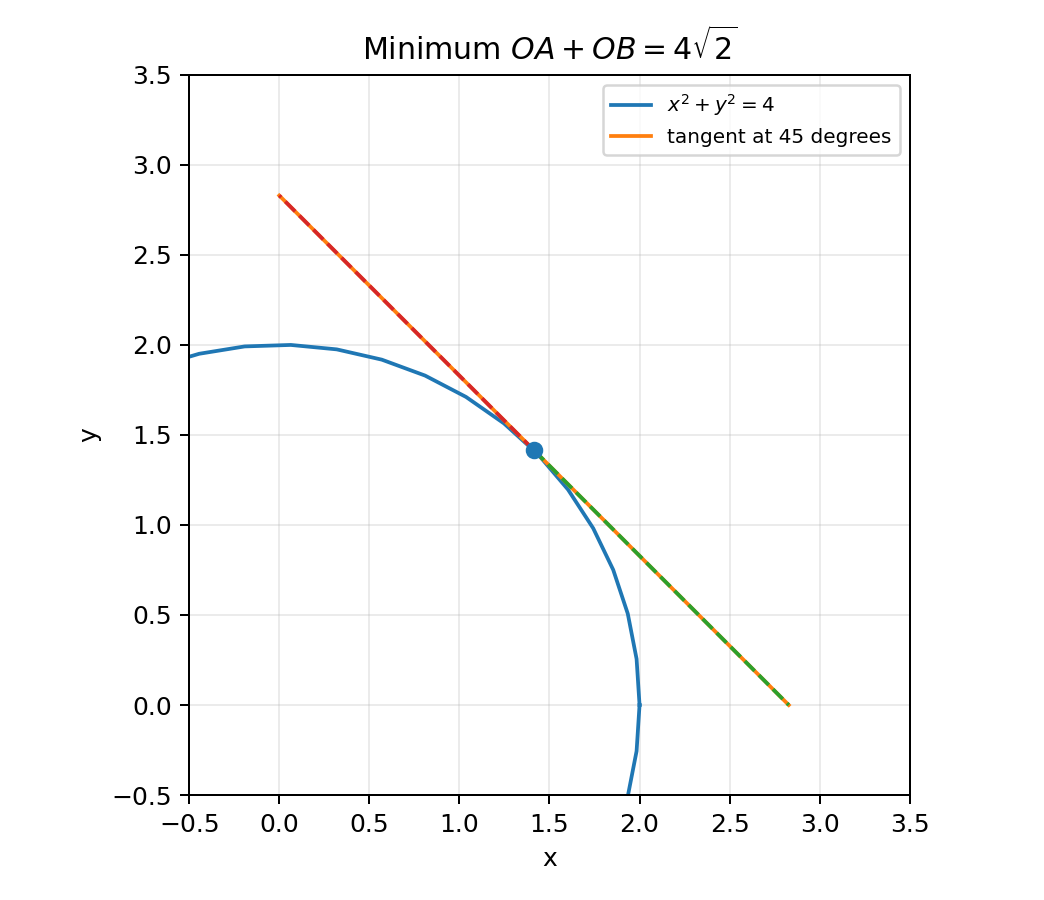
\includegraphics[width=0.92\linewidth]{../CBSE-2015-Class12-Updated-corrected_V3/figs/Q64_CircleTangent.png}\end{figure}
\par\smallskip
\noindent\textbf{Code reference -}
\par\noindent\fbox{\parbox{\dimexpr\linewidth-2\fboxsep-2\fboxrule\relax}{\centering\texttt{../CBSE-2015-Class12-Updated-corrected_V3/codes/Q64.py}}}
\par\smallskip

\setcounter{enumi}{64}\item Find the maximum area of an isosceles triangle inscribed in $\frac{x^2}{16}+\frac{y^2}{9}=1$ with its vertex at an end of the major axis.
\solution By symmetry, take the fixed vertex as $(4,0)$ and the other two vertices as $(u,v)$ and $(u,-v)$. From the ellipse, $v=3\sqrt{1-u^2/16}$. The area is
\[
A(u)=v(4-u)=3(4-u)\sqrt{1-u^2/16}.
\]
Differentiation gives $A'(u)=0$ when $u^2-2u-8=0$, i.e. $u=4$ or $u=-2$. The endpoint $u=4$ has zero area, so the maximum is at $u=-2$, where $v=3\sqrt3/2$. Thus
\[
A_{\max}=6\left(\frac{3\sqrt3}{2}\right)=9\sqrt3\qquad\eqref{eq:ellipse-area-65}.
\]
\begin{figure}[H]\centering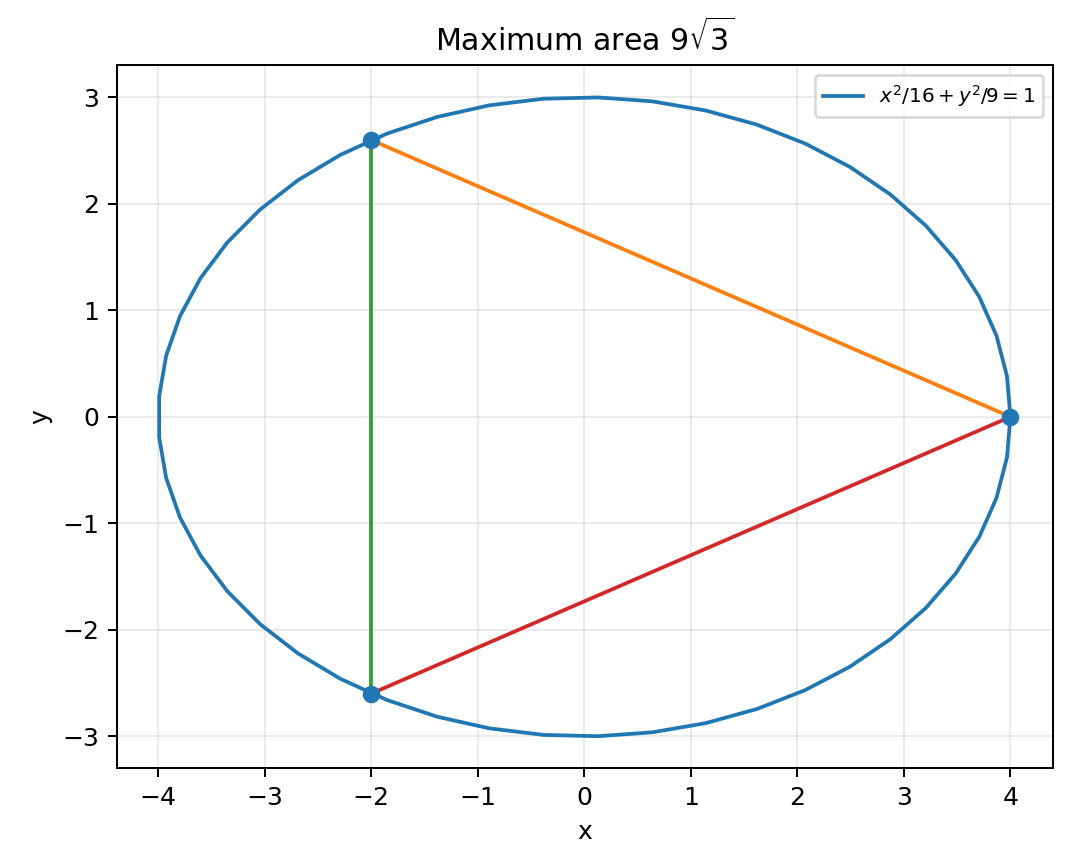
\includegraphics[width=0.92\linewidth]{../CBSE-2015-Class12-Updated-corrected_V3/figs/Q65_EllipseTriangle.png}\end{figure}
\par\smallskip
\noindent\textbf{Code reference -}
\par\noindent\fbox{\parbox{\dimexpr\linewidth-2\fboxsep-2\fboxrule\relax}{\centering\texttt{../CBSE-2015-Class12-Updated-corrected_V3/codes/Q65.py}}}
\par\smallskip\end{enumerate}

\end{document}
